%\documentclass[journal]{vgtc}                % final (journal style)
\documentclass[review,journal]{vgtc}         % review (journal style)
%\documentclass[widereview]{vgtc}             % wide-spaced review
%\documentclass[preprint,journal]{vgtc}       % preprint (journal style)

%% Uncomment one of the lines above depending on where your paper is
%% in the conference process. ``review'' and ``widereview'' are for review
%% submission, ``preprint'' is for pre-publication, and the final version
%% doesn't use a specific qualifier.

%% Please use one of the ``review'' options in combination with the
%% assigned online id (see below) ONLY if your paper uses a double blind
%% review process. Some conferences, like IEEE Vis and InfoVis, have NOT
%% in the past.

%% Please use the ``preprint''  option when producing a preprint version
%% for sharing your article on an open access repository

%% Please note that the use of figures other than the optional teaser is not permitted on the first page
%% of the journal version.  Figures should begin on the second page and be
%% in CMYK or Grey scale format, otherwise, colour shifting may occur
%% during the printing process.  Papers submitted with figures other than the optional teaser on the
%% first page will be refused. Also, the teaser figure should only have the
%% width of the abstract as the template enforces it.

%% These few lines make a distinction between latex and pdflatex calls and they
%% bring in essential packages for graphics and font handling.
%% Note that due to the \DeclareGraphicsExtensions{} call it is no longer necessary
%% to provide the the path and extension of a graphics file:
%% 
\includegraphics{diamondrule} is completely sufficient.
%%
\ifpdf%                                % if we use pdflatex
  \pdfoutput=1\relax                   % create PDFs from pdfLaTeX
  \pdfcompresslevel=9                  % PDF Compression
  \pdfoptionpdfminorversion=7          % create PDF 1.7
  \ExecuteOptions{pdftex}
  \usepackage{graphicx}                % allow us to embed graphics files
  \DeclareGraphicsExtensions{.pdf,.png,.jpg,.jpeg} % for pdflatex we expect .pdf, .png, or .jpg files
\else%                                 % else we use pure latex
  \ExecuteOptions{dvips}
  \usepackage{graphicx}                % allow us to embed graphics files
  \DeclareGraphicsExtensions{.eps}     % for pure latex we expect eps files
\fi%

%% it is recomended to use ``\autoref{sec:bla}'' instead of ``Fig.~\ref{sec:bla}''
\graphicspath{{figures/}{pictures/}{images/}{./}} % where to search for the images

\usepackage{microtype}                 % use micro-typography (slightly more compact, better to read)
\PassOptionsToPackage{warn}{textcomp}  % to address font issues with \textrightarrow
\usepackage{textcomp}                  % use better special symbols
\usepackage{mathptmx}                  % use matching math font
\usepackage{times}                     % we use Times as the main font
\renewcommand*\ttdefault{txtt}         % a nicer typewriter font
\usepackage{cite}                      % needed to automatically sort the references
\usepackage{tabu}                      % only used for the table example
\usepackage{booktabs}                  % only used for the table example
%% We encourage the use of mathptmx for consistent usage of times font
%% throughout the proceedings. However, if you encounter conflicts
%% with other math-related packages, you may want to disable it.


%% Regulus specific packages
\usepackage{scrextend}
\usepackage{calc}
\usepackage{enumitem}
\usepackage{todonotes}
% Select what to do with command \comment:
% \newcommand{\comment}[1]{}  %comment not showed
\newcommand{\comment}[2]
{\par {\bfseries \color{blue} [#2]: #1 \par}} %comment showed

\usepackage{algorithm}
\usepackage[noend]{algpseudocode}

\newcommand{\regulus}{\emph{Regulus}~}
\usepackage{listings}
\usepackage{xcolor}


%New colors defined below
\definecolor{codegreen}{rgb}{0,0.6,0}
\definecolor{codegray}{rgb}{0.5,0.5,0.5}
\definecolor{codepurple}{rgb}{0.58,0,0.82}
\definecolor{backcolour}{rgb}{0.95,0.95,0.92}

%Code listing style named "mystyle"
\lstdefinestyle{mystyle}{
% backgroundcolor=\color{backcolour},
  commentstyle=\color{codegreen},
  keywordstyle=\color{magenta},
  numberstyle=\tiny\color{codegray},
  stringstyle=\color{codepurple},
  basicstyle=\ttfamily\footnotesize,
  breakatwhitespace=false,
  breaklines=true,
  captionpos=b,
  frame=single,
  keepspaces=true,
%   numbers=left,
  numbersep=5pt,
  showspaces=false,
  showstringspaces=false,
  showtabs=false,
  tabsize=2
}
%"mystyle" code listing set
\lstset{style=mystyle}

%% In preprint mode you may define your own headline. If not, the default IEEE copyright message will appear in preprint mode.
%\preprinttext{To appear in IEEE Transactions on Visualization and Computer Graphics.}

%% In preprint mode, this adds a link to the version of the paper on IEEEXplore
%% Uncomment this line when you produce a preprint version of the article
%% after the article receives a DOI for the paper from IEEE
%\ieeedoi{xx.xxxx/TVCG.201x.xxxxxxx}

%% If you are submitting a paper to a conference for review with a double
%% blind reviewing process, please replace the value ``0'' below with your
%% OnlineID. Otherwise, you may safely leave it at ``0''.
\onlineid{0}

%% declare the category of your paper, only shown in review mode
\vgtccategory{Research}
%% please declare the paper type of your paper to help reviewers, only shown in review mode
%% choices:
%% * algorithm/technique
%% * application/design study
%% * evaluation
%% * system
%% * theory/model
\vgtcpapertype{algorithm/technique}

%% Paper title.
\title{Regulus}

%% This is how authors are specified in the journal style

%% indicate IEEE Member or Student Member in form indicated below
\author{Yarden Livnat%, \textit{Member, IEEE}
	, Dan Maljovec
	, Attila Gyulassy,
	, Valerio Pascucci
	}
\authorfooter{
%% insert punctuation at end of each item
\item
 Yarden Livnat is with the Scientific Computing and Imaging Institute at the University of Utah.
 E-mail: yarden@sci.utah.edu.
\item
 Dan Maljovec is with the xxx.
 E-mail:
 \item  Attila Gyulassy is with xxx.
 E-mail:
 \item
 Valerio Pascucci is with the Scientific Computing and Imaging Institute at the University of Utah.
 E-mail: pascucci@sci.utah.edu.
}

%other entries to be set up for journal
\shortauthortitle{Livnat \MakeLowercase{\textit{et al.}}: Global Illumination for Fun and Profit}
%\shortauthortitle{Firstauthor \MakeLowercase{\textit{et al.}}: Paper Title}

%% Abstract section.
\abstract{Understanding the response of an output variable to multi-dimensional inputs lies at the heart of many data exploration endeavours. Topology-based methods, in particular Morse theory and persistent homology, provide a useful framework for studying this relationship, as phenomena of interest often appear naturally as fundamental features. The Morse-Smale complex captures a wide range of features by partitioning the domain of a scalar function into piecewise monotonic regions, while persistent homology provides a means to study these features at different scales of simplification. Previous works demonstrated how to compute such a representation and its usefulness to gain insight into multi-dimensional data. However, exploration of the multi-scale nature of the data was limited to selecting a single simplification threshold from a plot of region count. In this paper, we present a novel tree visualization that provides a concise overview of the entire hierarchy of topological features. The structure of the tree provides initial insights in terms of the distribution, size, and stability of all partitions. We use regression analysis to fit linear models in each partition, and develop local and relative measures to further assess uniqueness and the importance of each partition, especially with respect parents/children in the feature hierarchy. The expressiveness of the tree visualization becomes apparent when we encode such measures using colors, and the layout allows an unprecedented level of control over feature selection during exploration. For instance, selecting features from multiple scales of the hierarchy enables a more nuanced exploration. Finally, we demonstrate our approach using examples from several scientific domains.
%
%Morse-Smale theory and persistence homology form a rich and powerful topology-based framework for studying complex high-dimensional scalar functions. A Morse-Smale complex captures a wide range of features by decomposing the scalar function into piecewise monotonic partitions while persistence homology provides a means for simplifying it at different levels of detail. Previous works focused on \textit{how} to create a simplified topological description for a given persistence value but provided only crude measures to help a user select an appropriate value from  ordered list of persistence values. 
%In this paper, we present a novel tree visualization that provides a concise hierarchical overview of all simplification steps with respect to their persistence levels. The overall structure of the tree provides initial insights in terms of the distribution, size and stability of all potential space partitioning. Rather than relying only on topological attributes, we use regression analysis to fit linear models in all potential partitions and develop local and relative measures to further assess uniqueness and the importance of each partition. The expressiveness of the tree visualization becomes apparent when we encode measures using colors and interact with one or more trees to guide the exploration of simplification space and the underlying function, and identify partitions of unique behavior. In addition, we discuss the notions of local and non-consistent simplifications using partitions from different persistence levels. Finally, we demonstrate our approach using examples from several scientific domains.
} 


%% Keywords that describe your work. Will show as 'Index Terms' in journal
%% please capitalize first letter and insert punctuation after last keyword
\keywords{Multidimensional data, Topology, Data exploration.}

%% ACM Computing Classification System (CCS).
%% See <http://www.acm.org/class/1998/> for details.
%% The ``\CCScat'' command takes four arguments.

%\CCScatlist{ % not used in journal version
% \CCScat{K.6.1}{Management of Computing and Information Systems}%
%{Project and People Management}{Life Cycle};
% \CCScat{K.7.m}{The Computing Profession}{Miscellaneous}{Ethics}
%}

%% A teaser figure can be included as follows
\teaser{
  \centering
  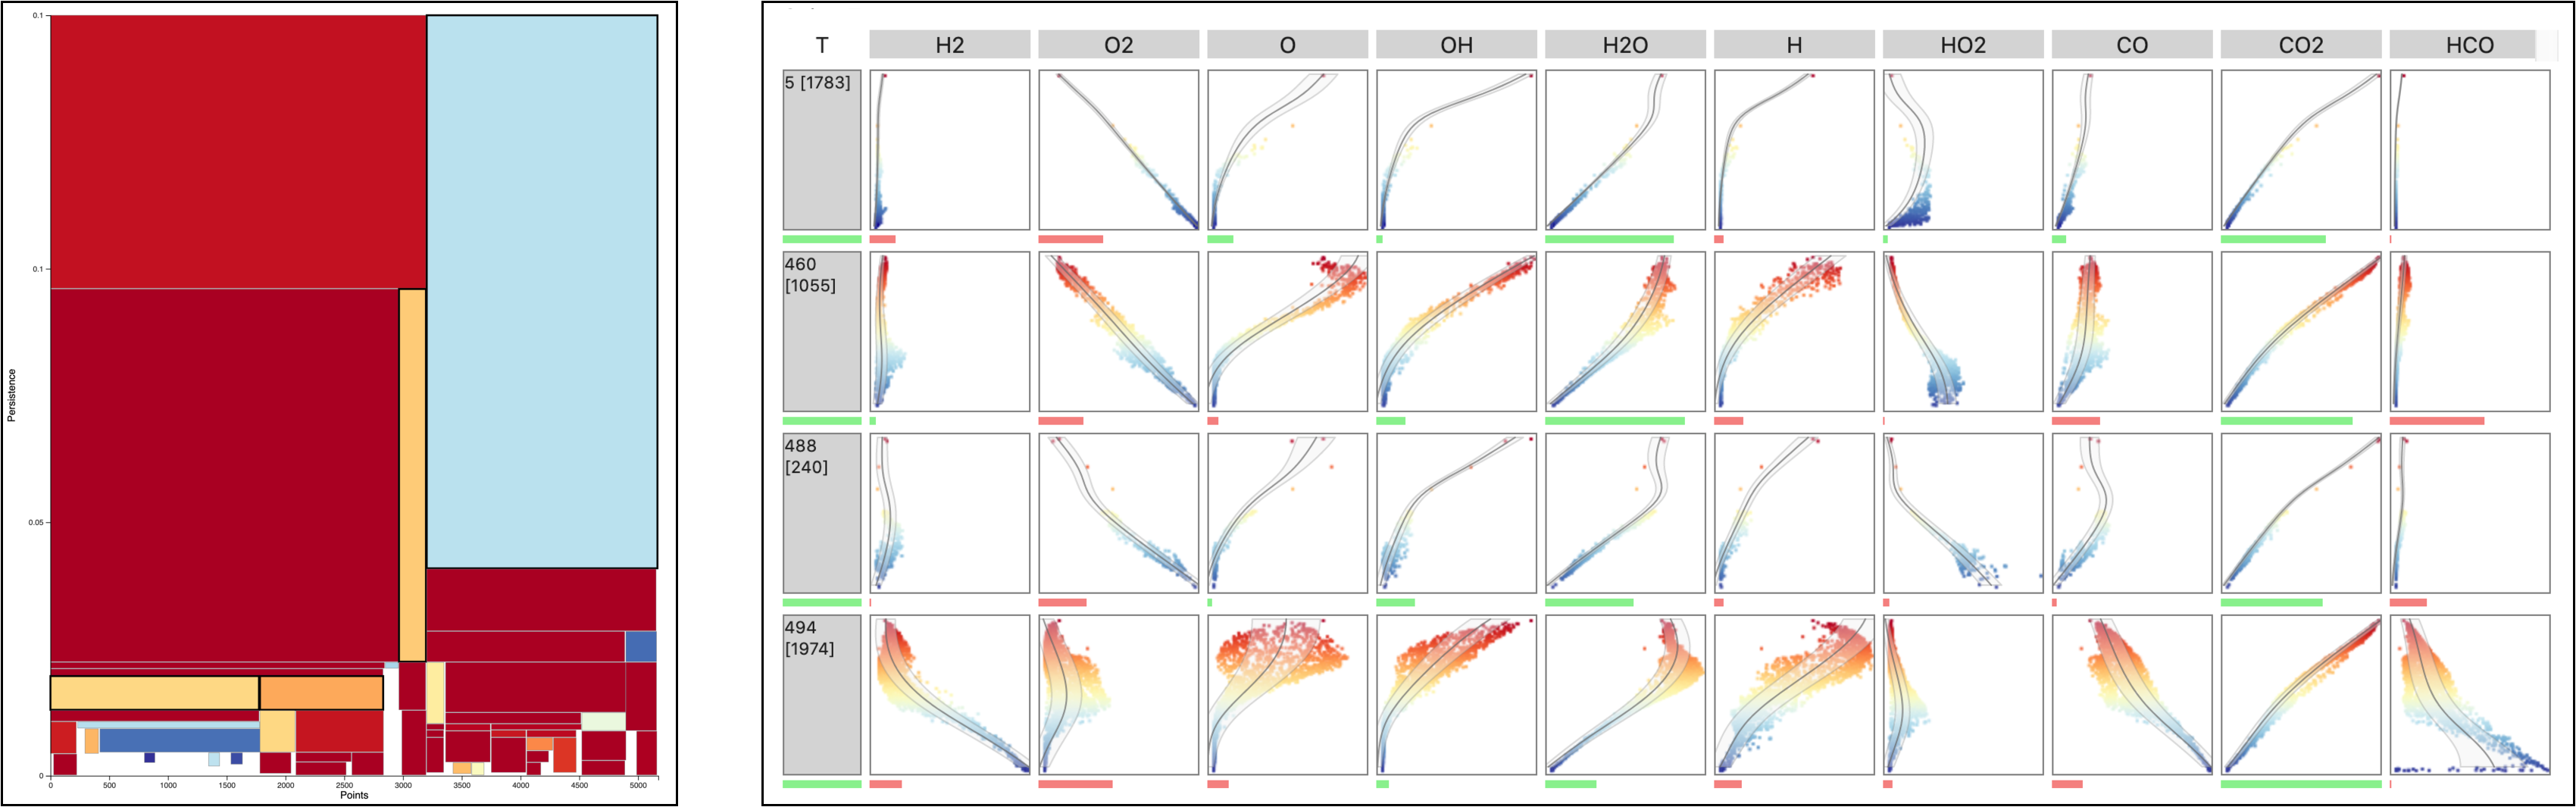
\includegraphics[width=\linewidth]{figs/teaser}
  \caption{Regulus}
  \label{fig:teaser}
}

%% Uncomment below to disable the manuscript note
%\renewcommand{\manuscriptnotetxt}{}

%% Copyright space is enabled by default as required by guidelines.
%% It is disabled by the 'review' option or via the following command:
% \nocopyrightspace


\vgtcinsertpkg

%%%%%%%%%%%%%%%%%%%%%%%%%%%%%%%%%%%%%%%%%%%%%%%%%%%%%%%%%%%%%%%%
%%%%%%%%%%%%%%%%%%%%%% START OF THE PAPER %%%%%%%%%%%%%%%%%%%%%%
%%%%%%%%%%%%%%%%%%%%%%%%%%%%%%%%%%%%%%%%%%%%%%%%%%%%%%%%%%%%%%%%%

\begin{document}

%% The ``\maketitle'' command must be the first command after the
%% ``\begin{document}'' command. It prepares and prints the title block.

%% the only exception to this rule is the \firstsection command
%\firstsection{Introduction}

%\maketitle

%% \section{Introduction} %for journal use above \firstsection{..} instead
%This template is for papers of VGTC-sponsored conferences such as IEEE VIS, IEEE VR, and ISMAR which are published %as special issues of TVCG. The template does not contain the respective dates of the conference/journal issue, these %will be entered by IEEE as part of the publication production process. Therefore, \textbf{please leave the copyright %statement at the bottom-left of this first page untouched}.
%
\firstsection{Introduction}
\maketitle
\label{sec:intro}

Many phenomena in science and engineering can be described by how an output variable depends on input parameters. For example, understanding the correlation between temperature and chemical species and turbulence in a computationally model of a combustion reaction can lead to better fuel or engine designs. As another example, understanding how the measured strength of concrete varies with the ratios of its ingredients can lead to more error-tolerant mixtures. Computational models are used to study such real-world phenomena, either by conducting computer simulations or through a set of well-designed experiments. Analysis of the results can then be used to improve the models, find optimal solutions, uncover unknown relationships, and support decision-making.

The set of relationships between inputs and output can be very specialized; for any input parameter, its relationship to the output variable may be conditioned on the variation in the other parameters. Topology provides a means of studying the shape of a function; for instance, identifying how local minima and maxima are related to each other both spatially and in terms of local importance. The Morse-Smale complex, in particular, decomposes the domain into monotonic regions that enable reasoning about local trends that contribute to the formation of a local maximum or minimum. In contrast to a user-defined query or hypercube sample, the topological partitions are intrinsic to the function and underlying manifold, and are well-suited for regression analysis. 

Local perturbations, artifacts of meshing, or small features can derail analysis, as it is difficult to separate phenomena from noise. Persistent homology describes topological features in terms of their life-span of the element from its birth critical point to its death in a sweep of the range of the function. In many applications, features below a persistence threshold are discarded as noise, a process that involves guesstimating an appropriate value, sometimes with the help of a persistence curve. In many applications, however, features appear with varying persistence in the domain. In multi-dimensional data analysis, in particular, justifying a simplification threshold is difficult as, until now, there have not been effective visualization and exploration techniques to understand the specific relationships between features at different scales. 

We introduce a novel visualization that is composed of a nested space-filling tree layout to visualize the topological hierarchy whose geometry encodes the size and persistence of topological features. We reinterpret persistence simplification hierarchies of the Morse-Smale complex as a merging tree of partitions, allowing an even finer granularity of feature selection than a single simplification operation and efficient layout. Color in the cells of the tree is used to encode one of many computed measures, such as fitness of a regression model to the corresponding topological feature, relationships between the models of parents and children, or any other computed attributes. Our new visualization is deployed in an open exploration environment implemented in Python and JupyterLab extensions. Linked views enable dynamic feature selection for flexible analysis. We evaluate the utility of the approach with use cases in combustion and nuclear energy, where salient features are visible at a glance, that previously depended on an exhaustive search through the simplification parameter.
Specifically, our contributions are:
\begin{itemize}[nosep]
    \item A new interpretation of persistence simplification of a Morse-Smale complex as a merger tree of partitions,

    \item A new visualization of topological hierarchies that encodes the size and life-span of every feature at once,

    \item Measures on topological features that incorporate the ancestry of a partition to aid and guide users in selecting the topological scale for analysis, 

    \item A user interface that enables adaptive simplification, and non-uniform and non-consistent selection of features across multiple scales, 
    
    \item Design of an open exploration environment to facilitate exploratory analysis. 
\end{itemize}


% \begin{itemize}[topsep=0cm, itemsep=0ex, parsep=0cm]
%     \item Computational models are used to study real-world phenomena, either by conducting computer simulations or a set of well-designed experiments. Give examples.
    
%     \item Analysis of the results can then be used to improve the models, find optimal solutions, uncover unknown relationships and support decision-making.
        
%     \item One important aim is to understand the shape of the output function. What are the local min and max values, where are they located and how are they associated with each other. Where are the min and max, how stable the function is at various location.
    
%     \item Another important aspect is understanding the behaviour of the function, that is the relationship between the input parameters and the output.
    
%     \item In particular, identifying regions of interest where the output function has unique characteristics or behavior with respect to the input parameters. Understanding the characteristics of the function in these ROI and around certain critical points.
    
%     \item These analysis can be done on the output function or on derived quantities.
    
%     \item Topology
    
%     \begin{itemize}
%         \item Morse-Smale and hierarchical simplification to deal with noise.
        
%          \item Geometric Skeleton: inverse relationships indicating which combinations of inputs are responsible for which output.
     
%         \item Topology data analysis (or is it Morse-Smale approaches?) tools often focus on on extrapolating $f$ at various refinement levels.
%     \end{itemize}

%     \item Simulation Ensembles
%     \todo[inline]{maybe this shouldn't be in the paper}

% \end{itemize}

% \item In this paper we focus on scalar functions. We use MSC theory to define local approximation of the function rather than a complete global one. 

% \begin{itemize}
%     \item Help an analyst identify regions of interest (partitions) in the input space, where the $f$ exhibit consistent behaviour. 
    
%     \item Note that in general these that ROI need not be hyper cubes.

%     \item While the function is defined on a manifold embedded in $R^d$, we do not aim to identify the manifold. 
    
%     \item from Gerber:
%     \textit{"We are not aiming to interpolate or extrapolate f , but to analyze and visualize its structure using the existing samples to provide insight into the relationship between the input parameters and the output"}. 

%     \item Explore the space of all potential simplifications to help the user select the appropriate refinement. Previous approaches rely on the user to select an appropriate refinement level based on crude measures, i.e. the focus is on \textit{What} to do given a persistence level. In contrast, we focus on the \textit{Why} question, i.e., why should the user select a particular refinement level, and should there be only global refinement level. 
    
%     \item we propose that other measures, in addition to persistence, can and should be used. These measure can describe attributes of a partition as well as relationships between partitions. Measures can depends on the data in the current partition,  multiple partitions or even on an (potentially temporal) ancestry relation.
    
%     \item An open exploration environment to facilitate the analysis exploration. It is designed to be used in a Notebook within a JupyterLab environment and as such our approach is designed for users that are knowledgeable with Python although it is simple to construct preconfigure setups for non programmers at a price of a closed system. The environment is open in the sense that it is meant to be integrated into a user's analysis workflow. Users can drive the UI from Python or by other components and can connect the UI to drive other tools, such as running additional simulations.s

% \end{itemize}

% \item Contributions
% \begin{itemize}
%     \item Regulus Tree: A new interpretation of a persistence refinement of a Morse-Smale complex as a set of nested partitions. \textbf{This need to be rephrased.}

%     \item A visualization approach that provides a global view over all potential simplifications  

%     \item Analysis of the nested partitions with respect to measures that are not necessarily geometric. 

%     \item Non-uniform and non-consistent simplifications
    
%     \item An open exploration environment to facilitate the analysis exploration. 
% \end{itemize}


\section{Background}
\label{sec:bg}

\subsection{Simulation Ensembles}
Exploring parameter space of simulation models.
\begin{itemize}
    \item ParaGlide~\cite{Bergner13} is a visualization system designed for interactive exploration of parameter spaces of multidimensional simulation models. Provides an informative design study and characterization of the domain. It aims to help guide data generation using a region-based user interface for parameter sampling and then dividing the model's input parameter space into partitions that represent distinct output behavior. Input space partition is done as a Cartesian product of ranges in the various input dimensions. The work focus on multiple output or derived measures.
    
    \item He et al.~\cite{He2020} employed a neural network to support parameter space exploration for ensemble simulations that are visualized in situ. They developed a convolutional regression model to learn a mapping from simulation and visualization parameters to visualization results. With the trained model, users can generate new images for different simulation parameters under various visualization settings. The work focuses on synthesizing images rather than of direct analysis of the the data
\end{itemize}

\subsubsection{Visual Steering}
\cite{Matkovic14, Splechtna15, Matkovic18}

\subsection{Topological Analysis}
Chazal~\cite{Chazal11}

\subsection{Morse Theory}
\label{sec:morse}
Morse~\cite{morse63}, Timo~\cite{Timo04}

Merge trees: expand. Giving a value, a merge tree can be used to extract a level set or segment the data but removing all the points below the given value. Merge trees were also used for visual exploration.

\subsection{Morse-Smale Approximation}
\label{sec:morse-smale}
Edelsbrunner~\cite{Edelsbrunner03}


\subsection{Visual Exploration}
\label{sec:hd-exploration}

\begin{itemize}
    \item Gerber 2010 work (this work is based on it). 
    \begin{itemize}
        \item Fit an inverse regression curve in each crystal to provide some sort of geometric summary. The curves are 1d curves in $R^d$ and in order to display them, Gerber project the curves down to 3d based on a PCA of all the data points.
        
        \item Once the user selects a persistence value using (\autoref{fig:persistence-ui}),  Gerber extracts the Morse-Smale representation of the data and then display all the inverse curves (see \autoref{sec:curve-fitting}) for in the partitions (crystals) in the 3D view.
        
        \item The 3D is problematic because 
            \begin{itemize}
                \item confusing - the axis are not clear and the twists in the curves don't provide any meaningful info
                \item to be meaningful the curves suppose to meet at the ends, which require some fiddling with the data. 
                \item the curves are not a good representation for coarse partitions that do not have a good linear model. 
            \end{itemize}
        
        \item the user can see details only about a single partition at a time
        
        \item single global refinement (persistence) level based on \autoref{fig:persistence-ui}
    
    \end{itemize}

    \item Dan's works. 
    \begin{itemize}
        \item Dan uses only linear lines instead of inverse regression curves because they are too expensive to precompute as Gerber did
        \item explain the views
        \item what are important aspects should be outlined here?
    \end{itemize}
    
    \item Use a persistence diagram \cite{Cohen-Steiner07}. Provides overall view of a MSC/MS but without connectivity between points. Does not address hierarchical MSC approximations.
\end{itemize}


\begin{figure}[htb]
    \begin{center}
     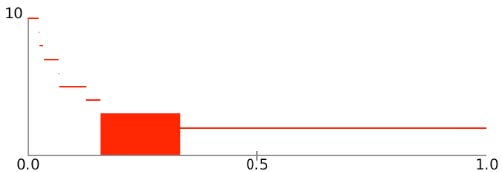
\includegraphics[width=\linewidth]{persistence-ui}
    \caption{Persistence curve showing the number of partitions as a function of persistence.}
    \label{fig:persistence-ui}
    \end{center}
\end{figure}


    \caption{Persistence curve showing the number of partitions as a function of persistence.}


\section{Regulus}
\label{sec:motivation}

While topological structures such as contour trees, merge trees and Morse-Smale complexes 
%are based on the function value at the critical points. It is important to note that while they do 
can capture features at multiple scales,
%and are often used to facilitate progressive simplifications, 
they nevertheless do not describe the simplification process, nor do they provide an overview of all the simplified topologies; rather, each instance describes, and is used to explore, only one simplified topology. Conceptually, simplification consist of creating a series of progressively coarse variation of one of these topological structures. In practice, only one model is created and then transformed to describe the required simplification level.
Visual exploration methods~\cite{Gerber10, maljovec16} are also designed to visualize one simplified topology at a time. Often, phenomena of interest appear at different scales in the data, and a single simplification threshold is insufficient for analysis.
The question of why should the user select a \textit{particular} simplification level was mostly left to the user's best estimation. 

In this work, we focus on the 'why' question in the context of using multi-dimensional Morse-Smale complexes  to study the relationships between input parameters and the output function. Rather than develop a method to find an optimal simplification threshold, our approach is to develop a visual representation of the whole persistence space that can help guide the user exploration. The new visualization, called Regulus Tree, is based on an interpretation of the simplification process in terms of nested partitions rather than cancellation on critical points. The expressiveness of the \RT comes to light when various attributes and measures are encoded on top of it. Another consideration of our design is to empower users to define their own attributes and measures and enable on the fly modification. The \RT enables,
% \begin{itemize}[itemsep=0pt]

    \noindent \textbf{Noise:} identify regions where noise is prominent
    
    \noindent  \textbf{Persistence level:} gain better understanding of the plateaus in terms of the size and stability of the partitions involves. Compare the statistical characteristics on the set of partitions for different persistence levels
    
    \noindent  \textbf{Adaptive simplification}: Select multiple persistence levels for individual features to adapt the simplification based on amount of relative rather than absolute noise, adapt to the local scale of features, and other measures of interest
    
    \noindent  \textbf{Local properties:} Compute and display local attributes of the function in different regions
    
    \noindent  \textbf{Relative measures:} Compare and contrast partitions from different locations in the function space as well as from different levels of details (persistence levels)
    
    \noindent  \textbf{Uniqueness:} Identify and study partitions that exhibit unique characteristics
    
    \noindent  \textbf{Clarity:} The \RT provide a hierarchical view of the persistence space in terms of nested partitions, which our collaborator scientists found much easier to grasp and comprehend as opposed to the technical description in terms of critical points cancellations. 
% \end{itemize}

In the following, we present the conceptual design, structure, and layout of the {\RT} as well as ways to simplify the tree itself. We describe several ways the \RT can be used for various tasks along with additional supporting views. We then introduce the notion of dynamic attributes and measures and show how they can provide unique insights and help guide the user exploration.

\section{Analysis \todo{Rephrase}}
\label{sec:analysis}
The Regulus tree depicts the hierarchical structure. We use the color to encode the value of a selected attribute in each node. 
 
\subsection{Attributes}
Each node has several core attributed such as the number of samples the partition contains or the min and max values of the function within the partition. One can potentially precompute additional attributes, such as the mean value, for each partition and store these values in the partition. One of the challenges of this approach is that precomputing all the attributes for all of the nodes can take a very long time. In addition, the user may not use or visualize all of these attributes during the analysis. Finally, the user may want to define new attributes on the fly, again, without precomputing them for each and every partition. 

Instead of precomputing attributes, we define an attribute by providing a factory function to compute its value for a given node and use a caching to compute the value only once when it is requested first. The function can requests other attributes from the tree. We describe our implementation in \autoref{sec:attr-impl}. \autoref{fig:attr-def} depicts a simple attribute definition.

\begin{lstlisting}[language=Python, float=htb, label=fig:attr-def, caption=Attribute definition]
def span(tree, node):
    return node.parent.data.persistence -
           node.data.persistence
tree.add_attr(span)
\end{lstlisting}


\subsection{Models}
We use linear regression to fit a linear model in each partition. There are many possible regression methods: Least squares, Ridge, Lasso, Elastic Net, Lars, etc. 

In general, other models, such as quadratic, can be use although they are more complex and in some sense defeat the purpose. A linear model for d-dimensional data requires d+1 parameters but a a quadratic models require 2 parameters per dimension (for $x_i$ and $x_i^2$) and well as all pairwise permutations $x_i \times x_j$ for a total of $d^2/2$ parameters.

\subsection{Measures}
\label{sec:measures}

\begin{description}
\item[Basic measures] span, min, max, normalize size

\item[Fitness] fitness of the local model to the local data. Note that this is an abstract operation that in general can be different for different models. Since we specify the model and measure independently the detail implementation can be left to the model. Example: \autoref{fig:fitness}

\item[Parent Fitness] the fitness of the parent model to the current node data. Explain why this is an important  measure.

\item[Child Fitness] the fitness of the current model to the data in the parent. Explain what is the purpose.

\end{description}


% \begin{figure*}[htb]
%     \begin{center}
%      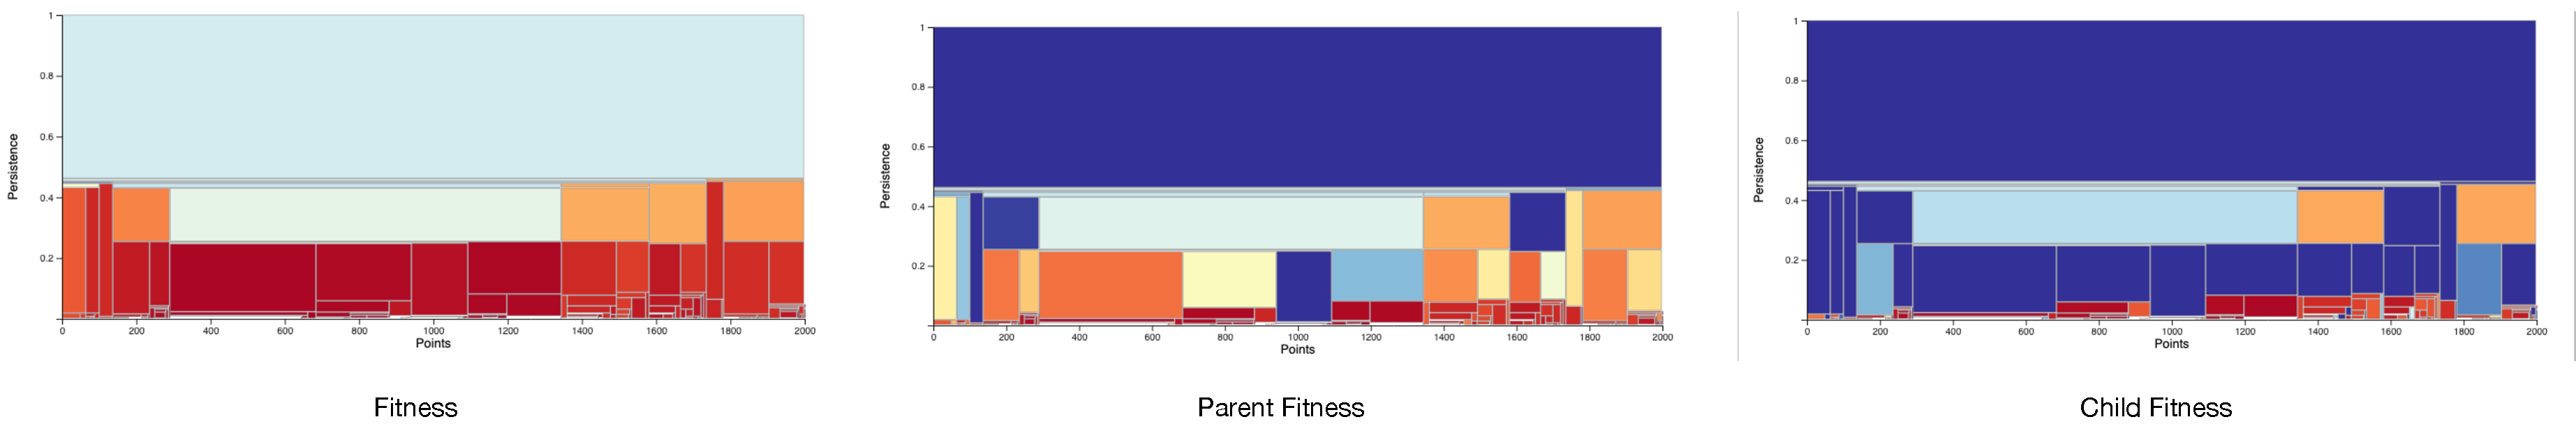
\includegraphics[width=\linewidth]{fitness}
%     \caption{Fitness of: a) local model to local data, b) parent model to local data, c) local model to parent data}
%     \label{fig:fitness}
%     \end{center}
% \end{figure*}
\subsubsection*{Example}
Consider ~\autoref{fig:details}
\begin{itemize}
    \item Root partition (id=0) has lowest fitness. 
    \item Partition 45 (bottom) represent the shallow hill (top left in the 3d view) which does not have a good linear model.
    \item Both partitions 21 and 34 have good linear models (0.944, 0.96) but their models are very different. 
    \item The parent partition (20) has a fitness of 0.770
    \item The Parent Fitness view (bottom right) demonstrates that the model for P0 moderately fit P21 (0.788) and P34 (0.651)
    \item The Child Fitness view (middle right) demonstrates that the models for P21 and P34 don't fit their parent P20 (0.224, -1.866) at all  
 \end{itemize}

% \begin{figure}[htb]
%     \begin{center}
%      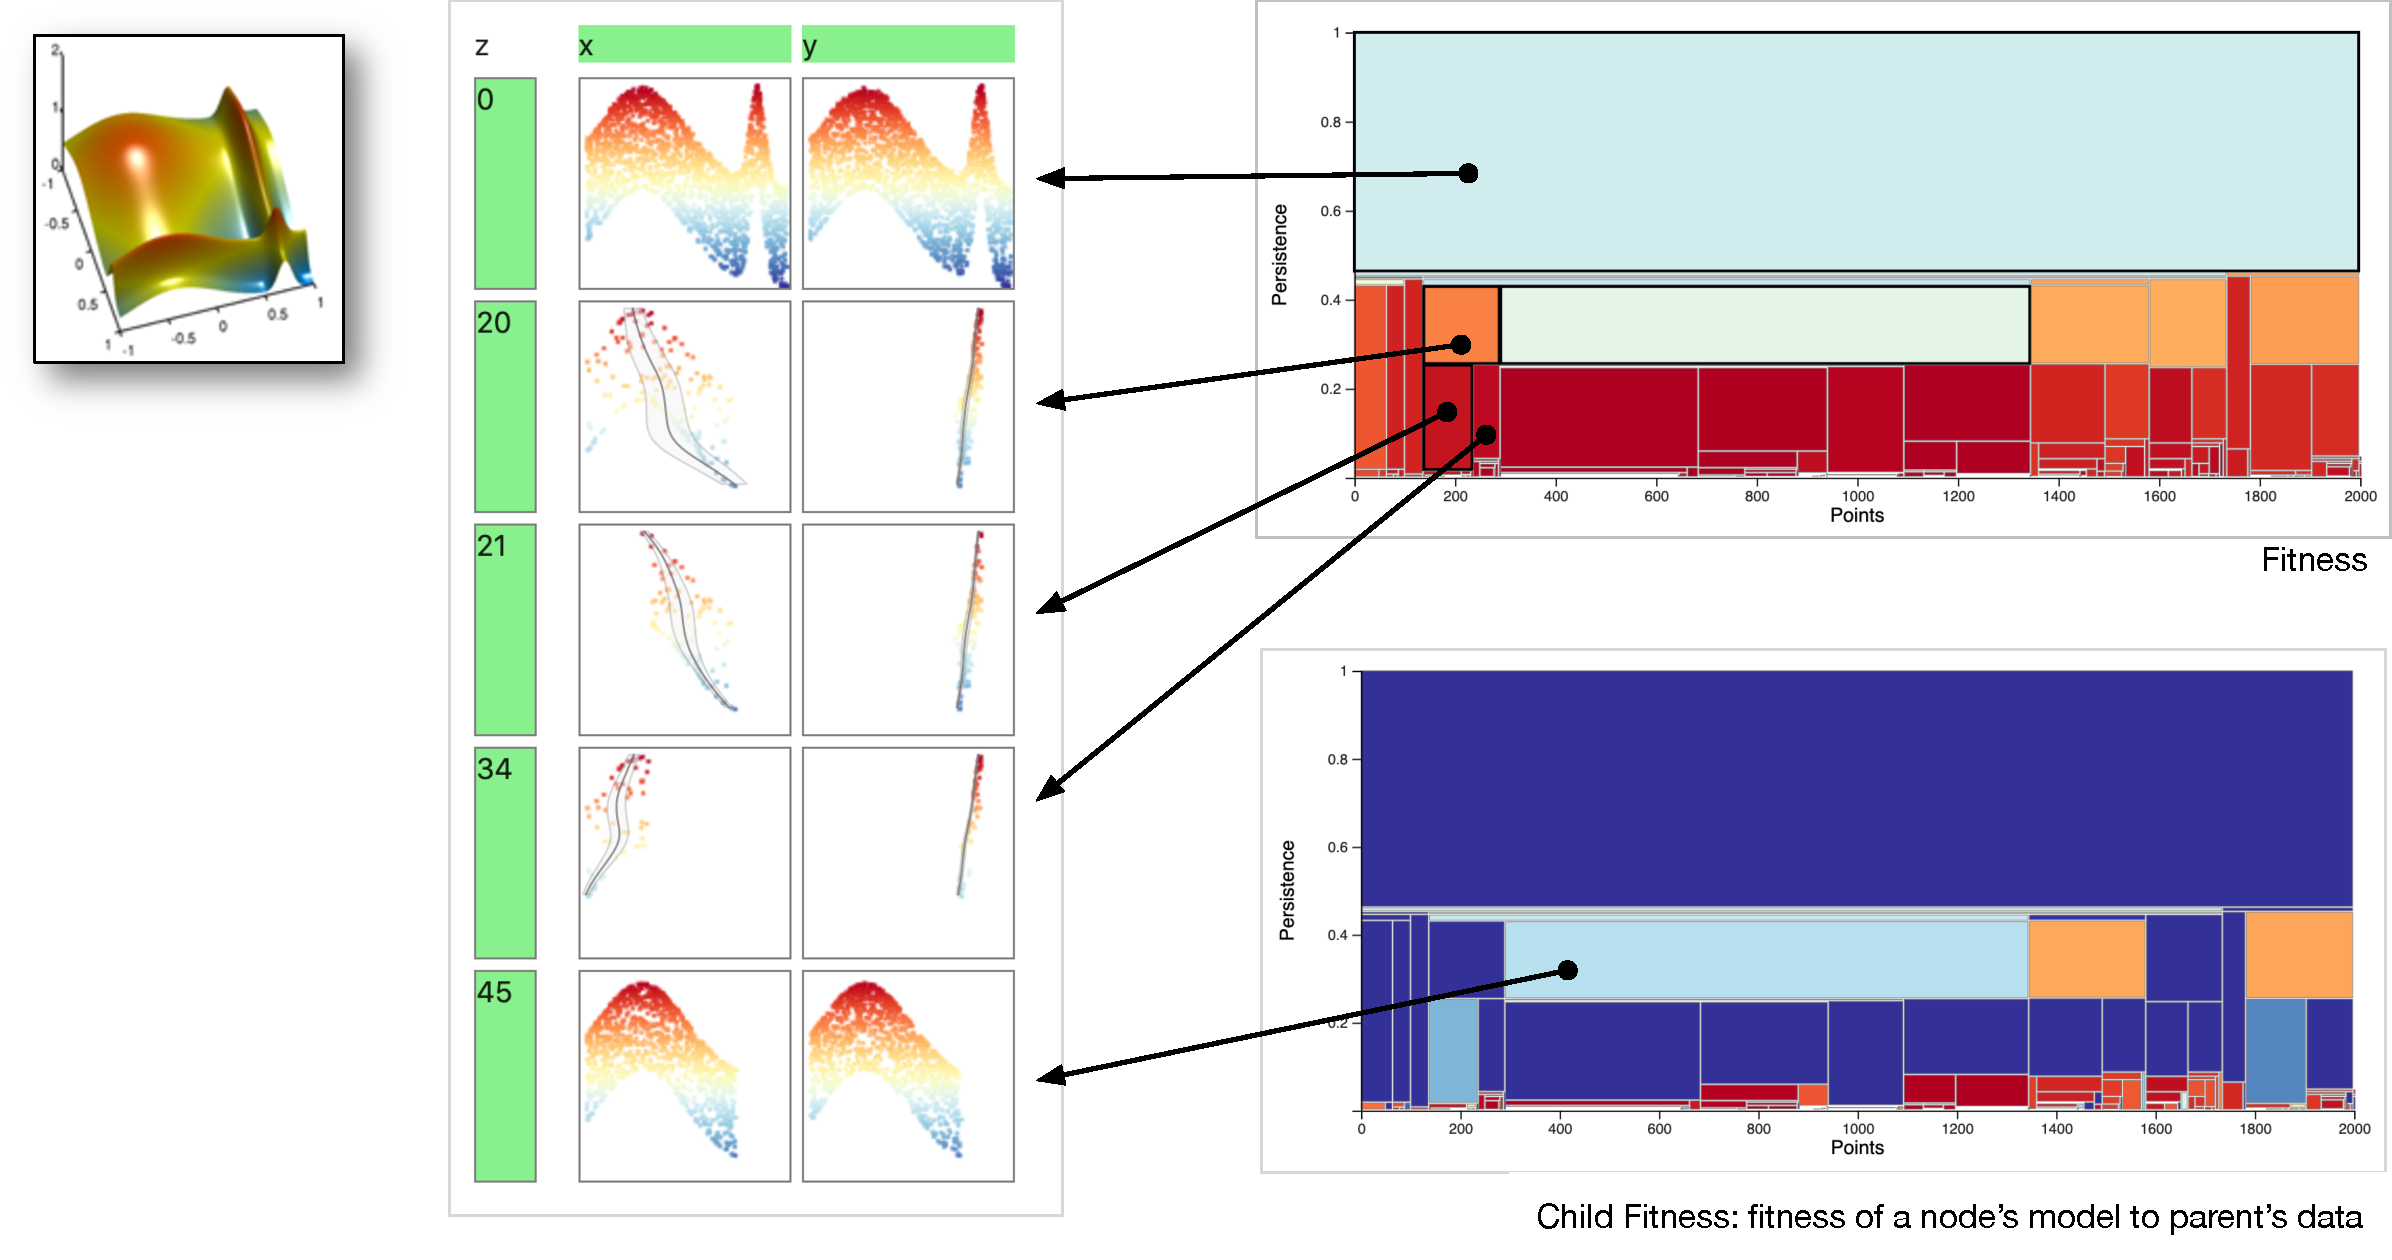
\includegraphics[width=\linewidth]{details}
%     \caption{Partitions Details: left A 3d view of the data. Middle: details view showing projected points for selected partitions. Right: A Regulus Tree where each nodes is colored based on the fitness of the local linear model to the data (red = 1, blue = 0)}
%     \label{fig:details}
%     \end{center}
% \end{figure}

\begin{figure}[thb]
    \begin{center}
     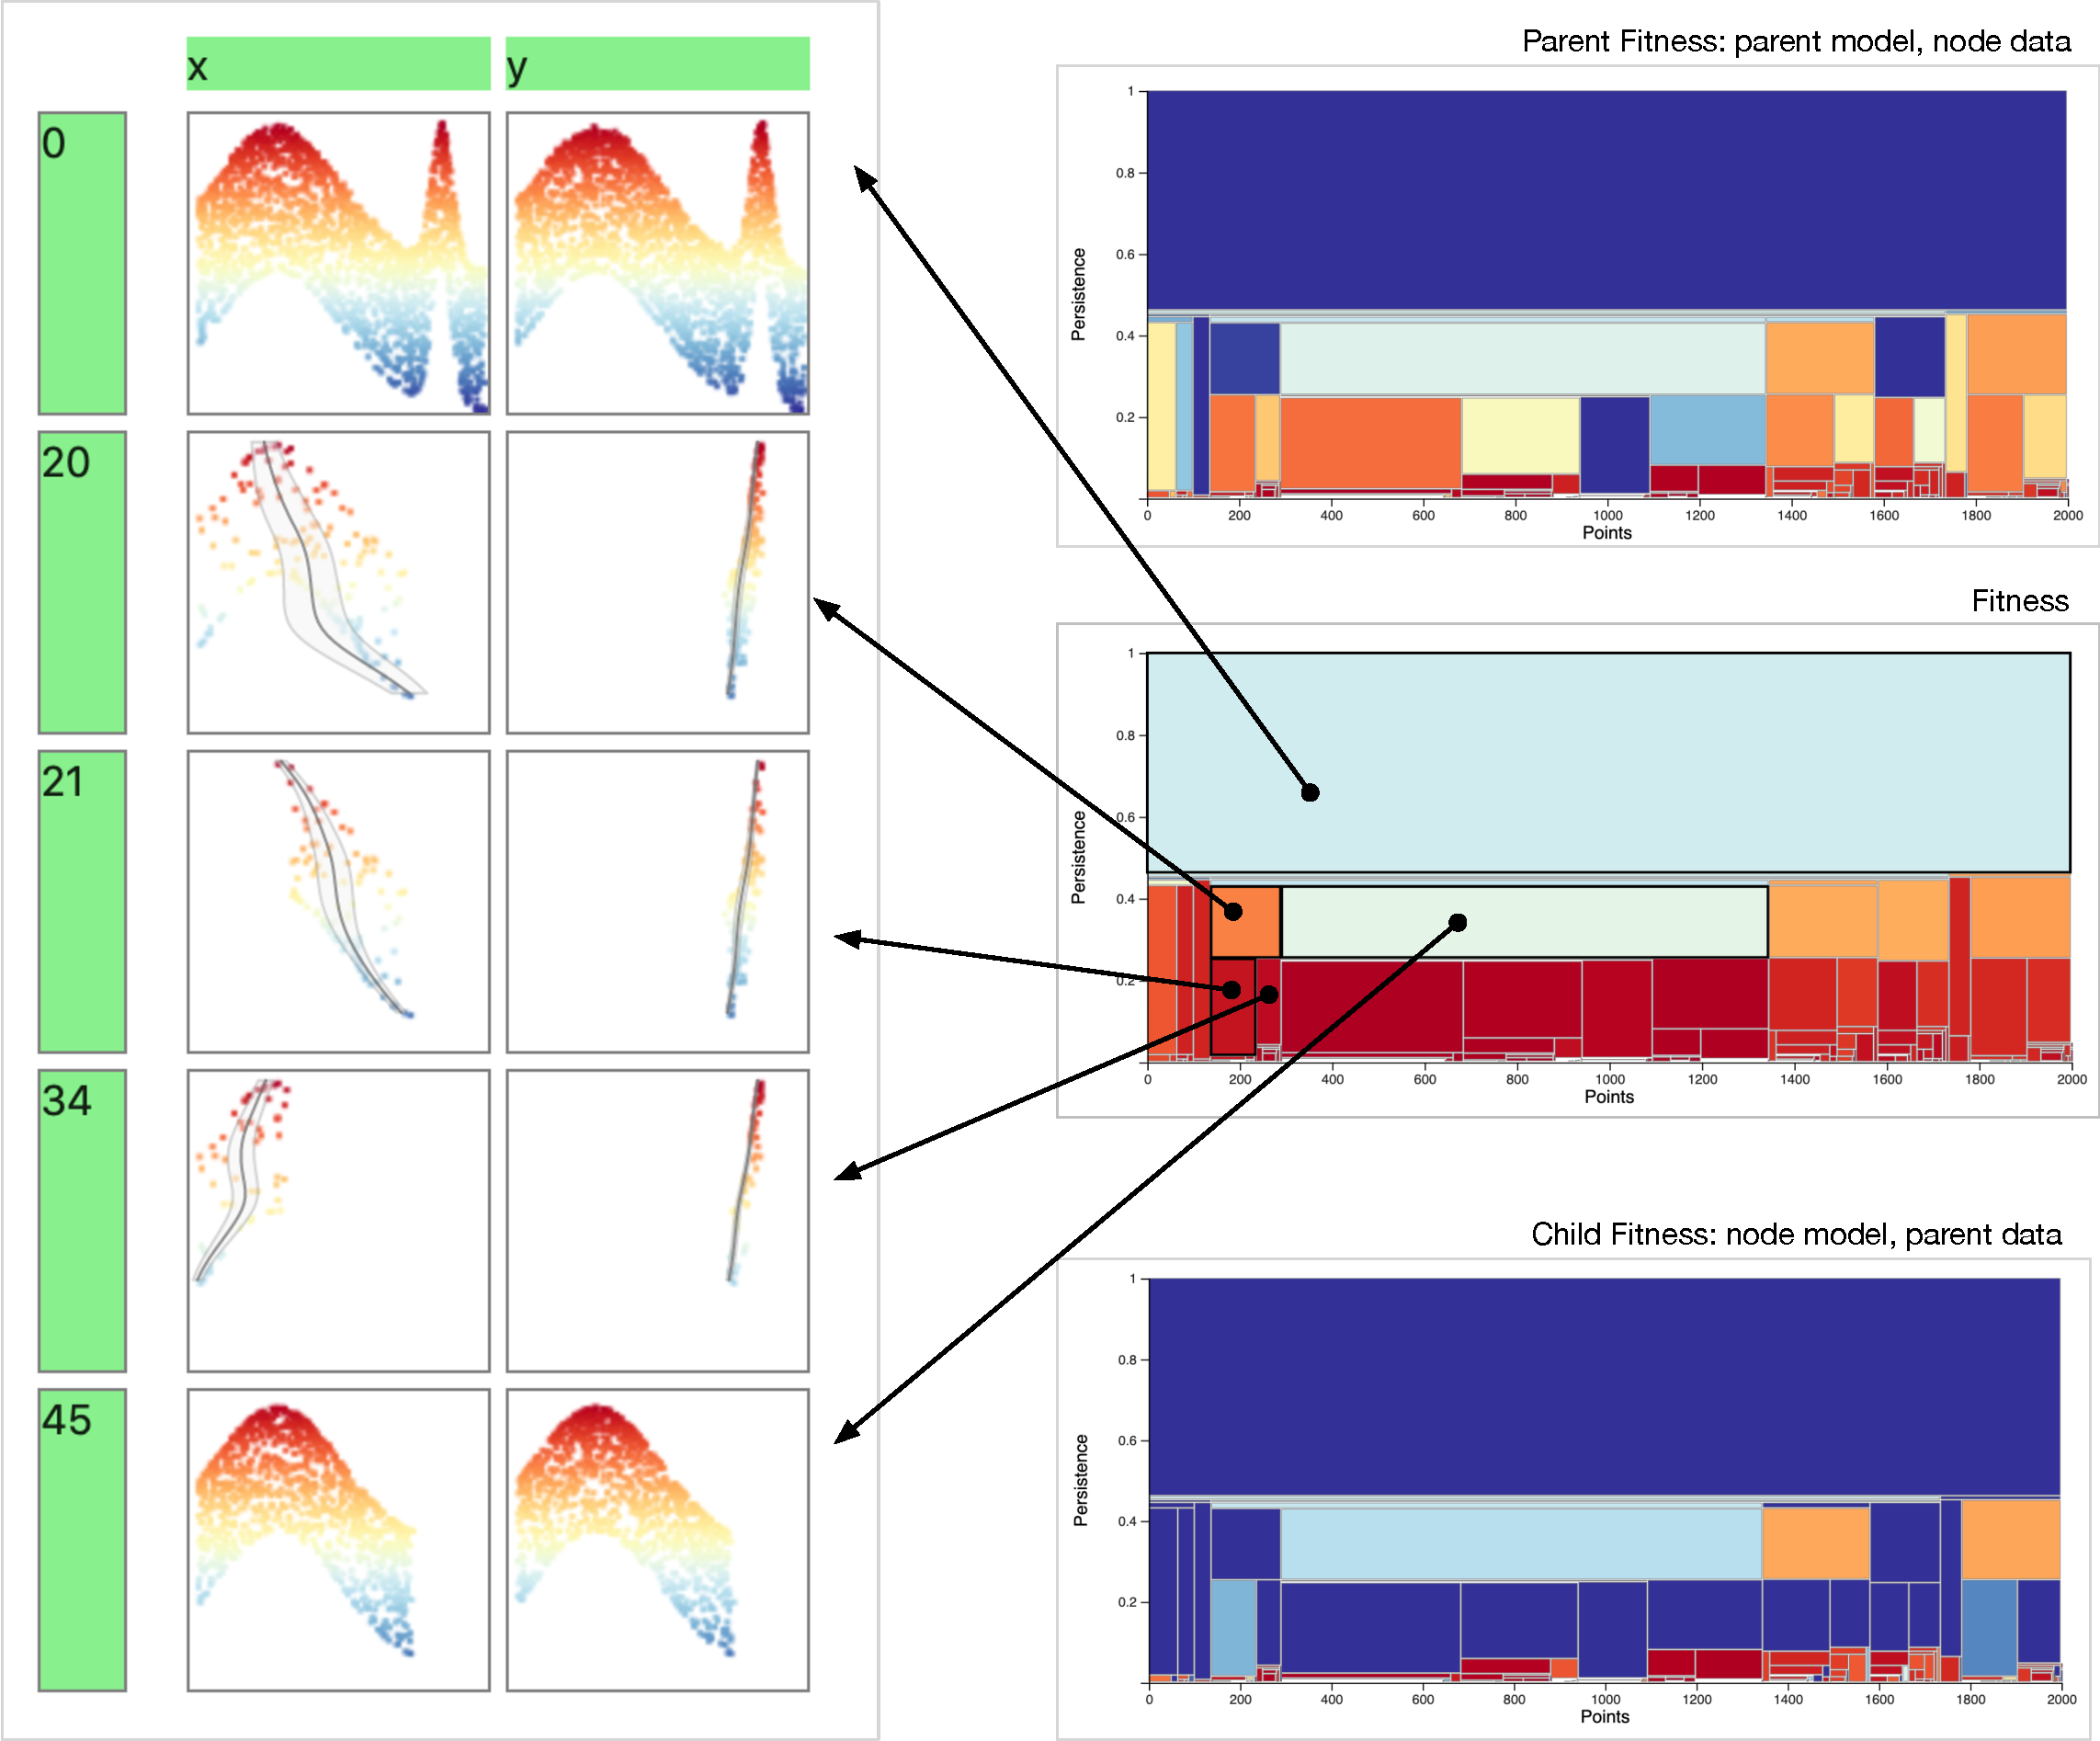
\includegraphics[width=\linewidth]{details-3}
    \caption{Left: details view showing points in selected partitions. Right: Three views of the Regulus Tree, each showing separate fitness measure (red = 1, blue = 0)}
    \label{fig:details}
    \end{center}
\end{figure}

\subsection{Inverse Regression Curves}
\label{sec:inverse-curves}

\begin{itemize}
    \item \textit{"Principal curves are smooth one-dimensional curves that pass through the middle of a p-dimensional dataset, providing a nonlinear summary of the data.They are non-parametric, and their shape is suggested by the data"}~\cite{Tibshirani92}
    \item Gerber~\cite{Gerber10} employed inverse regression curves based on locally weighted regression (LOWESS)~\cite{Cleveland88}. He used the mean std to define a hyper tube around the inverse curve (hyper circle with radium = mean std).
\end{itemize}

Gerber used the inverse regression curves to provide a geometric summary of a partition. For a given persistence level, Gerber displayed the inverse curves after projecting them to a 3D using PCA. This presentation often lead to confusion by users as they tried to assign meaning to the shape of the curves in 3D, which Gerber already noted shouldn't be done.

Describe LOWESSS.

We use the inverse regression curves in two ways. 
\begin{itemize}
    \item show in details view along with $\pm \sigma$, similar to Gerber
    \item use as a skeleton approximation of a partition and use it as a guide to select addition samples
\end{itemize}

\subsection{Sampling}
Choosing samples (partition, n, scale): 
\begin{enumerate}
    \item compute the inverse curve, I, and std deviation for the partition. The curve is computed at n points along the $y_{min} .. y_{max}$ attained in the given partition
    \item compute a hyper tube along the curve with hyper-rectangle cross section $\pm s \times sigma_i$ each dimension, where s is a scale given by the user 
    \item For each of control points of the curve along y, compute the area of the cross section. Normalize by the are of the tube this defines a pdf.
    \item select $k$ values of y using the pdf.
    \item for each selected $y^k$ choose $x_i^k \in [I_i - s \times \sigma, I_i + s \times \sigma]$ 
\end{enumerate}

We run a simulation for each sample. We can use the new data in two ways. First, we can compare each proposed sample with the computed one to evaluate how well our model prediction works. In this case we can add the computed sample to the partition but not reevaluate the MSC. Second, we can restart the whole process and evaluate a new MSC and Regulus decomposition. Note that in this case, the MSC will not necessarily be the same. This is a known issue with MSC and is beyond the scope of this work. 

\begin{figure}[thb]
    \begin{center}
     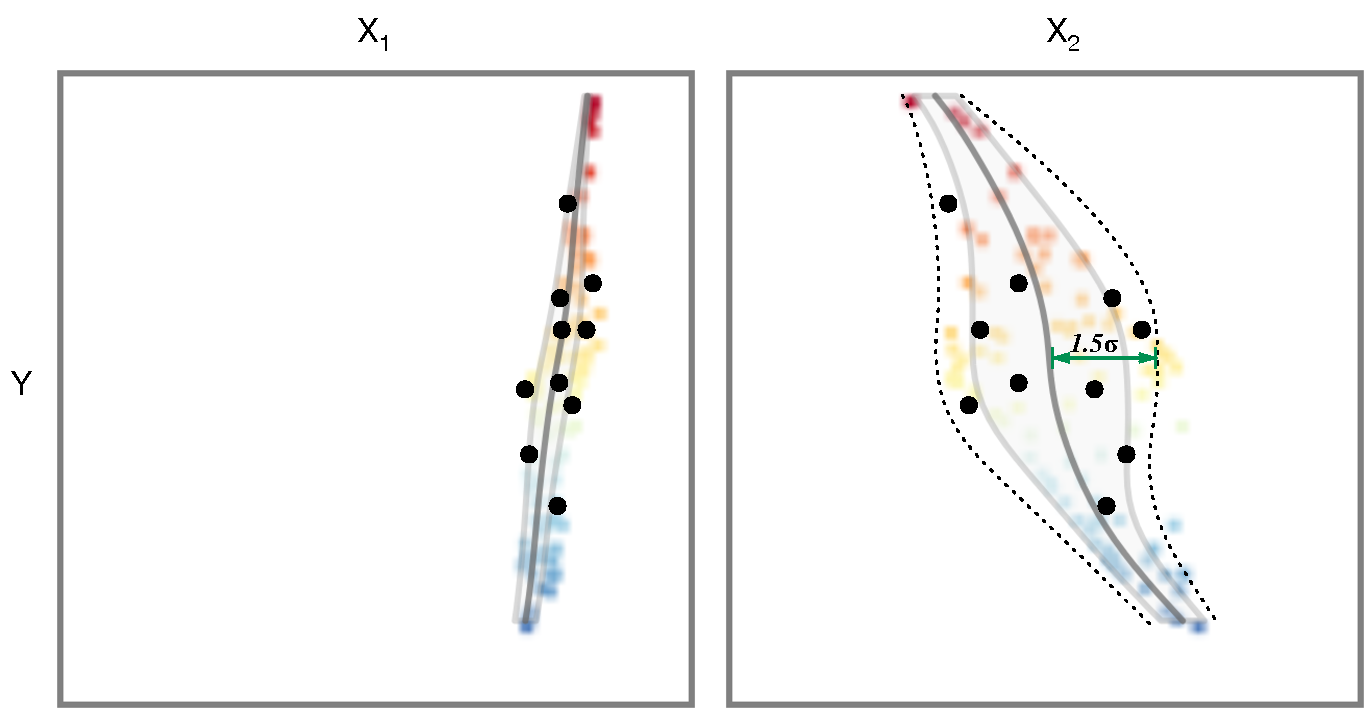
\includegraphics[width=\linewidth]{samples}
    \caption{Selecting samples using the inverse regression curves. The inverse curve is represented by the central gray curve. The two light gray curves represent the area one $\sigma$ around the curve and the dash lines shows the sampling area defined by $s \times \sigma$ where $s$ is a scale given by the user.}
    \label{fig:samples}
    \end{center}
\end{figure}

\subsection{Tree Visibility and Simplification}

\subsubsection*{Nodes Visibility}
Focus on a subset of partitions without changing the tree structure, i.e. only hide irrelevant nodes. For example, focus only on partition with high model fitness but where the model does not fit the parent data well.

\subsubsection*{Tree Reduction}
Instead of hiding nodes one can remove them from the tree. 
One way it to prune the tree based on some criterion (filter). Alternatively, we can reduce the tree by removing individual nodes from the tree based on a given filter and changing the tree structure.


\begin{figure}[htb]
    \begin{center}
     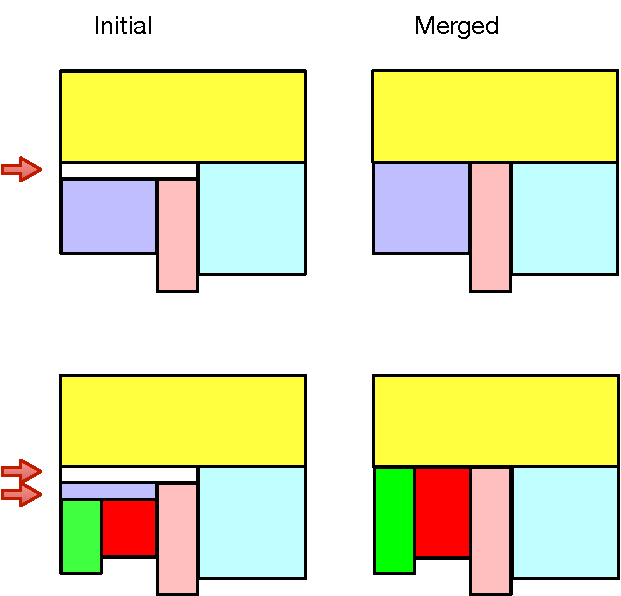
\includegraphics[width=\linewidth]{reduce}
    \caption{Regulus Tree Reduction}
    \label{fig:reduce}
    \end{center}
\end{figure}

\begin{figure}[htb]
    \begin{center}
     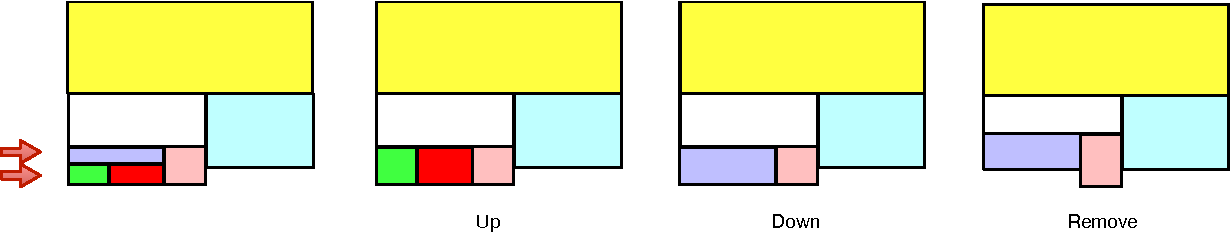
\includegraphics[width=\linewidth]{reduce-leaves}
    \caption{Regulus Tree Reduction at the leaves}
    \label{fig:reduce-leaves}
    \end{center}
\end{figure}
\section{Exploration Environment}
\label{sec:app}

Consider adding this section to describe the Regulus/IPyRegulus system.

Designed to facilitate an \textit{Analysis First} approach. Enable analysts to visualize data as part of their analysis workflow and employ their functions as models, measures and filters. 

\begin{figure}
    \centering
    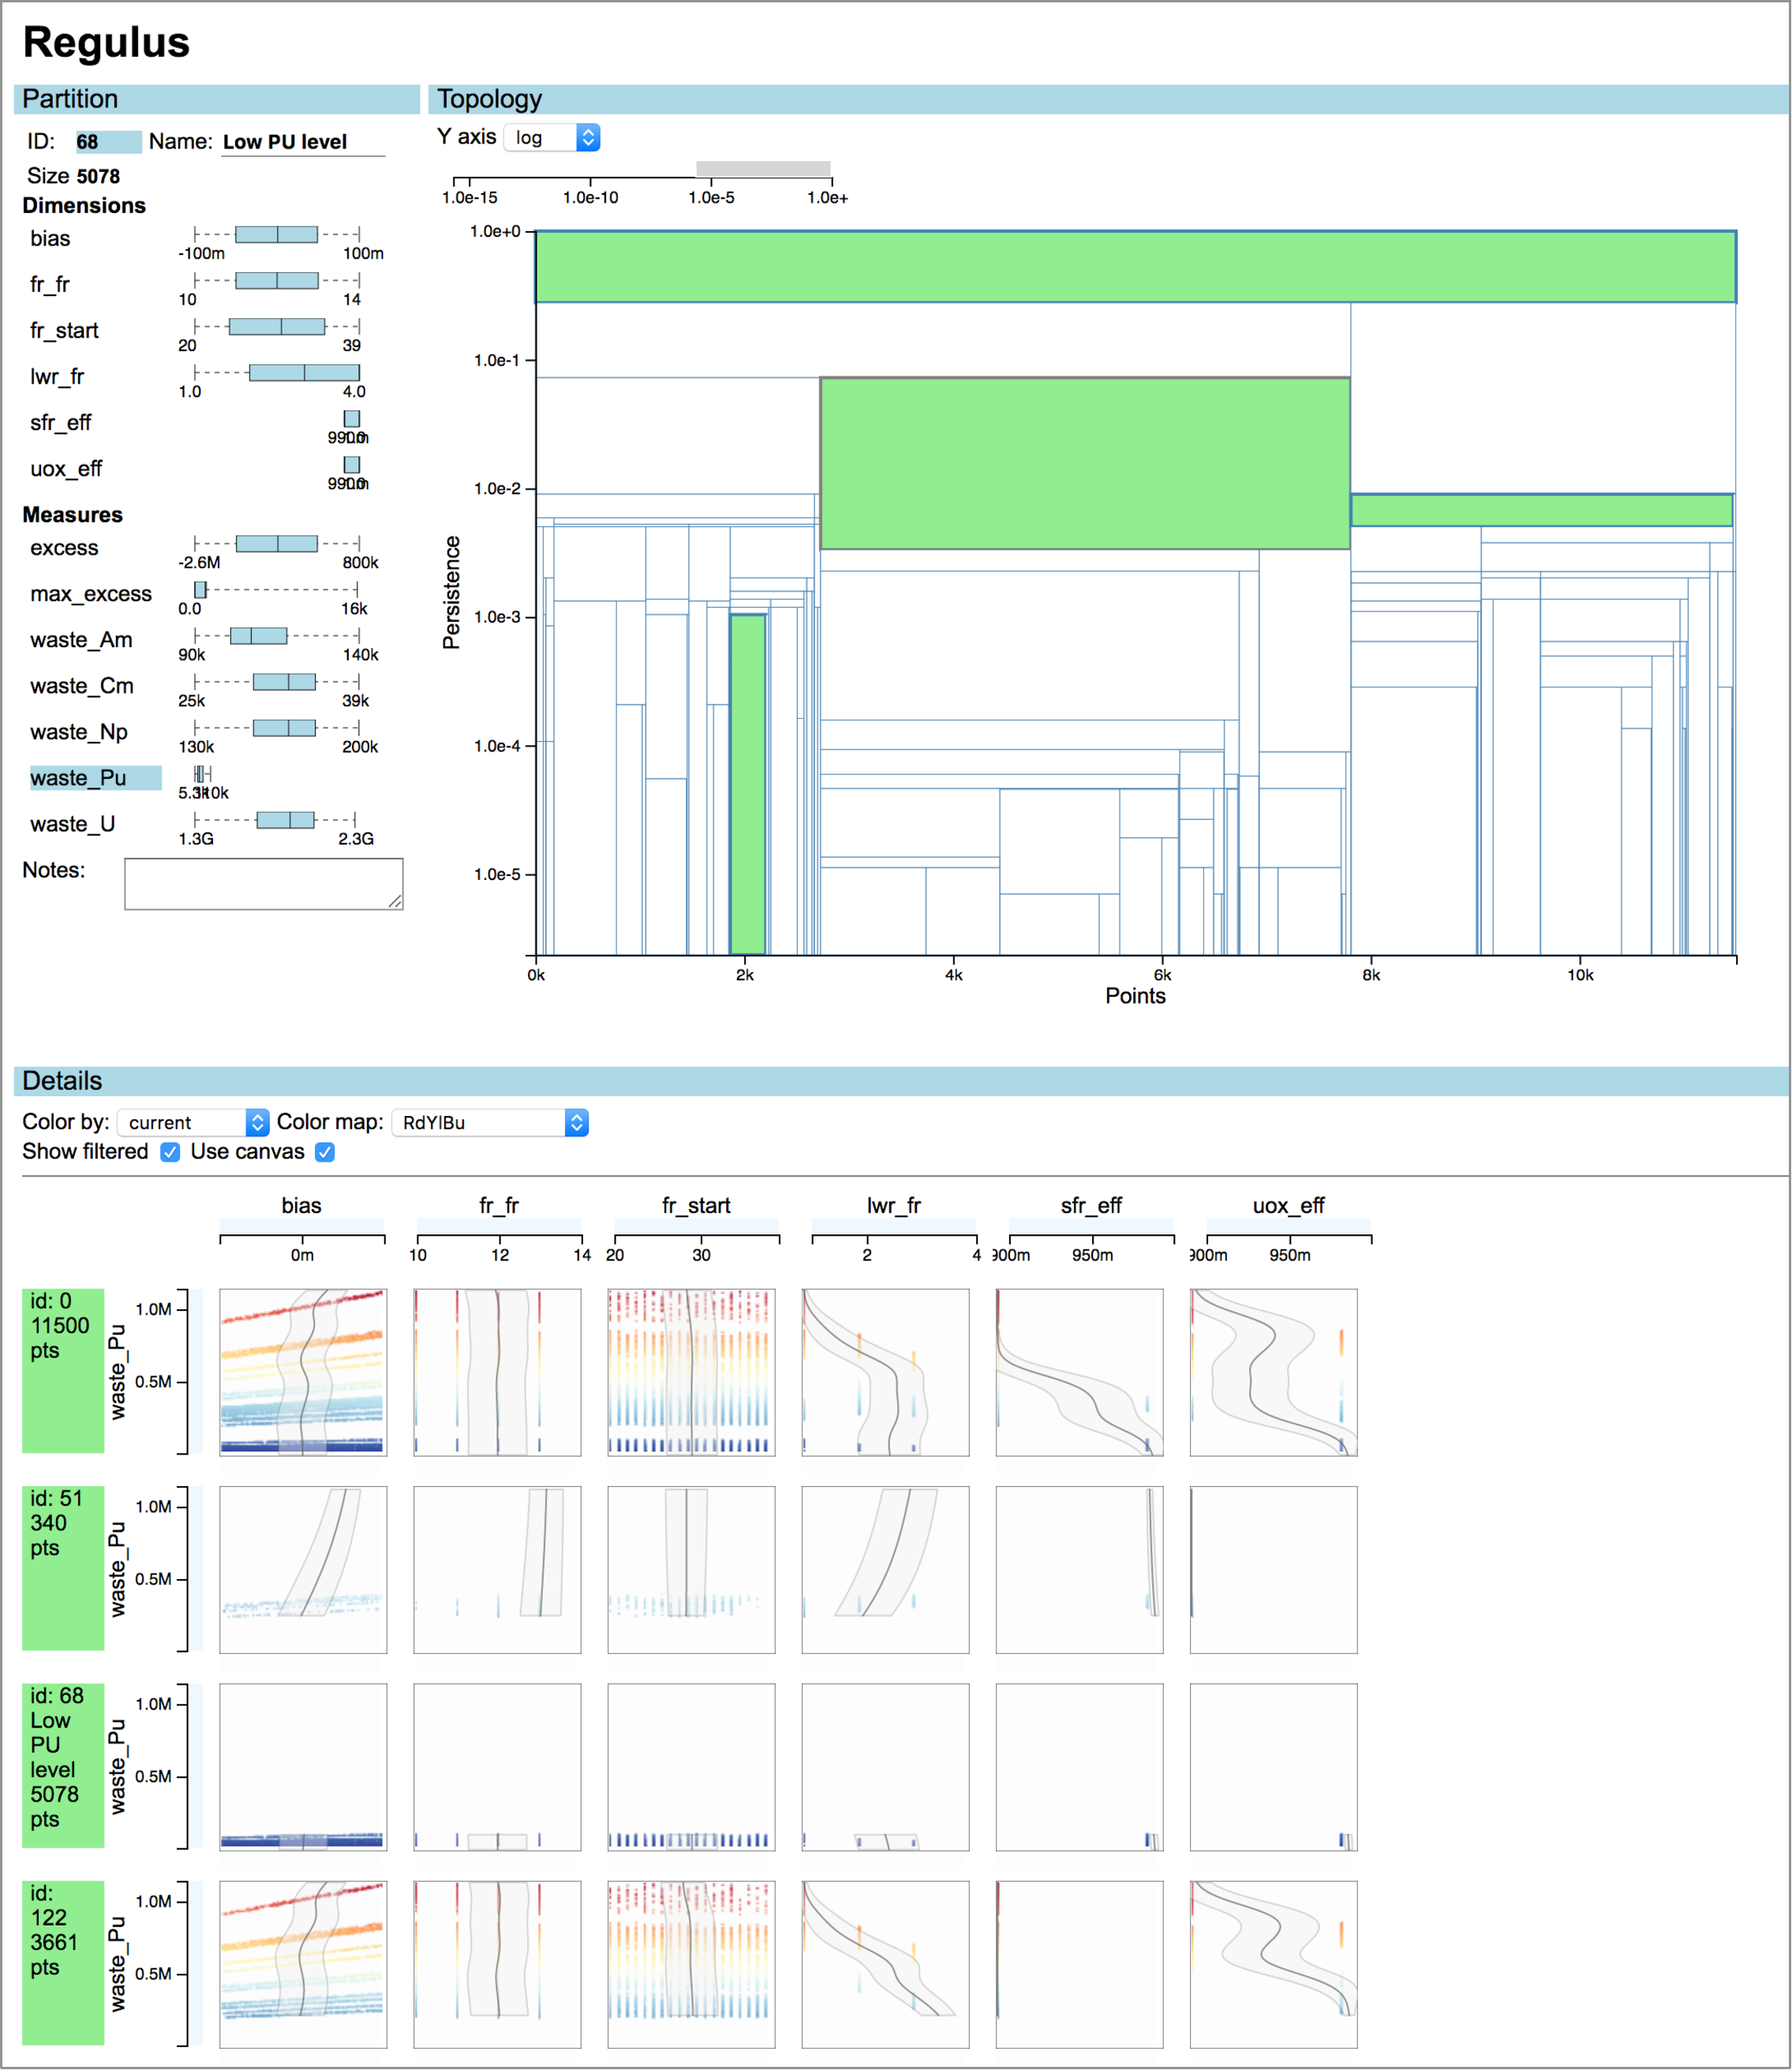
\includegraphics[width=\linewidth]{regulus-js}
    \caption{Visualization first implementation}
    \label{fig:regulus-js}
\end{figure}

Software consist of \textbf{Regulus}: a pure python package and \textbf{IPyRegulus}: interactive widgets for JupyterLab. 

\subsection{Regulus Attributes}
\label{sec:attr-impl}

\subsubsection{Caching}
\label{sec:caching}
Our aim is to avoid computing attributes, such as models and measures, for all the nodes. Instead, each attribute is associate with a generator function and a cache. An attribute value for a node will be computed using the generator function the first time it is requested and the value will be stored in the cache. If the user saves a Regulus object to a file, the generator function and the cached values will be saved in the file and will be loaded with the Regulus object the next time.

\begin{lstlisting}[language=Python, caption=Attributes can be used to reduce computations., float=htb, label='fig:model-fitness]
from sklearn import linear_model as lm

def linear_model(tree, node):
    model = lm.LinearRegresssion()
    model.fit(node.data.x, node.data.y)
    return model
    
def fitness(tree, node):
    model = tree['linear_model'][node]
    return model.score(node.data.x, node.data.y)
 
# Naive implementation 
# Not suitable for derived trees
# See Chained Attributes section
def parent_fitness(tree, node):
    parent_model = tree['linear_model'][node.parent]
    return parent_model.score(node.data.x, 
                              node.data.y)
    
tree.add_attr(linear_model)
tree.add_attr(fitness)
tree.add_attr(parent_fitness)
\end{lstlisting}

\subsection{Chained Attributes}
\label{sec:chained_attrs}

A Regulus tree may be derived from another, such as when one tree is a simplification of another (see \autoref{sec:simplification}). We want to avoid computing attributes for the derived tree that were already implemented in the original tree such a node fitness. However, some attributes depends on the tree structure.  

\begin{lstlisting}[language=Python, 
    caption=Chained attributes. Parent/child relation depends on the current tree structure, float=htb, label=fig:relative-fitness]

def relative_fitness(tree, has_model, has_pts):
    return tree['linear'][has_model].score(has_pts.data.x, has_pts.data.y)
    
def parent_fitness(tree, node):
    return tree['relative_fitness'][node.parent, node]

def child_fitness(tree, node):
    return tree['relative_fitness'][node, node.parent]    
\end{lstlisting}

\subsection{IPyRegulus}
\label{sec:ipyregulus}

A set of visualization widgets in a jupyter notebook and in particular in JupyterLab.

Discuss the benefits of using a notebook:
\begin{itemize}
    \item linear order
    \item repeatably
    \item scripted
\end{itemize}

A single model can be viewed several times. 

We want to avoid moving the data (points) and the Regulus structure (partitions) for each view. 

\begin{description}
\item[DataWidget] represents a model of the data and all the Morse-Smale partitions 
\item[DetailsView] refers to a DataWidget for points
\item[TreeWidget] represents a Regulus Tree and a set of attributes that were requested for visualization. Has not data points. A model with no visualization
\item[TreeView] refers to a TreeWidget for the tree structure.
\end{description}

\subsubsection{Side Panel}
\label{sec:sidepanel}
The need for a side panel that can be controlled by the user (add, resize, collapse views).

\subsubsection{Coordinated Multiple Views}
\label{sec:cmv}

See \autoref{fig:cmv}.

\begin{figure}[htb]
    \begin{center}
     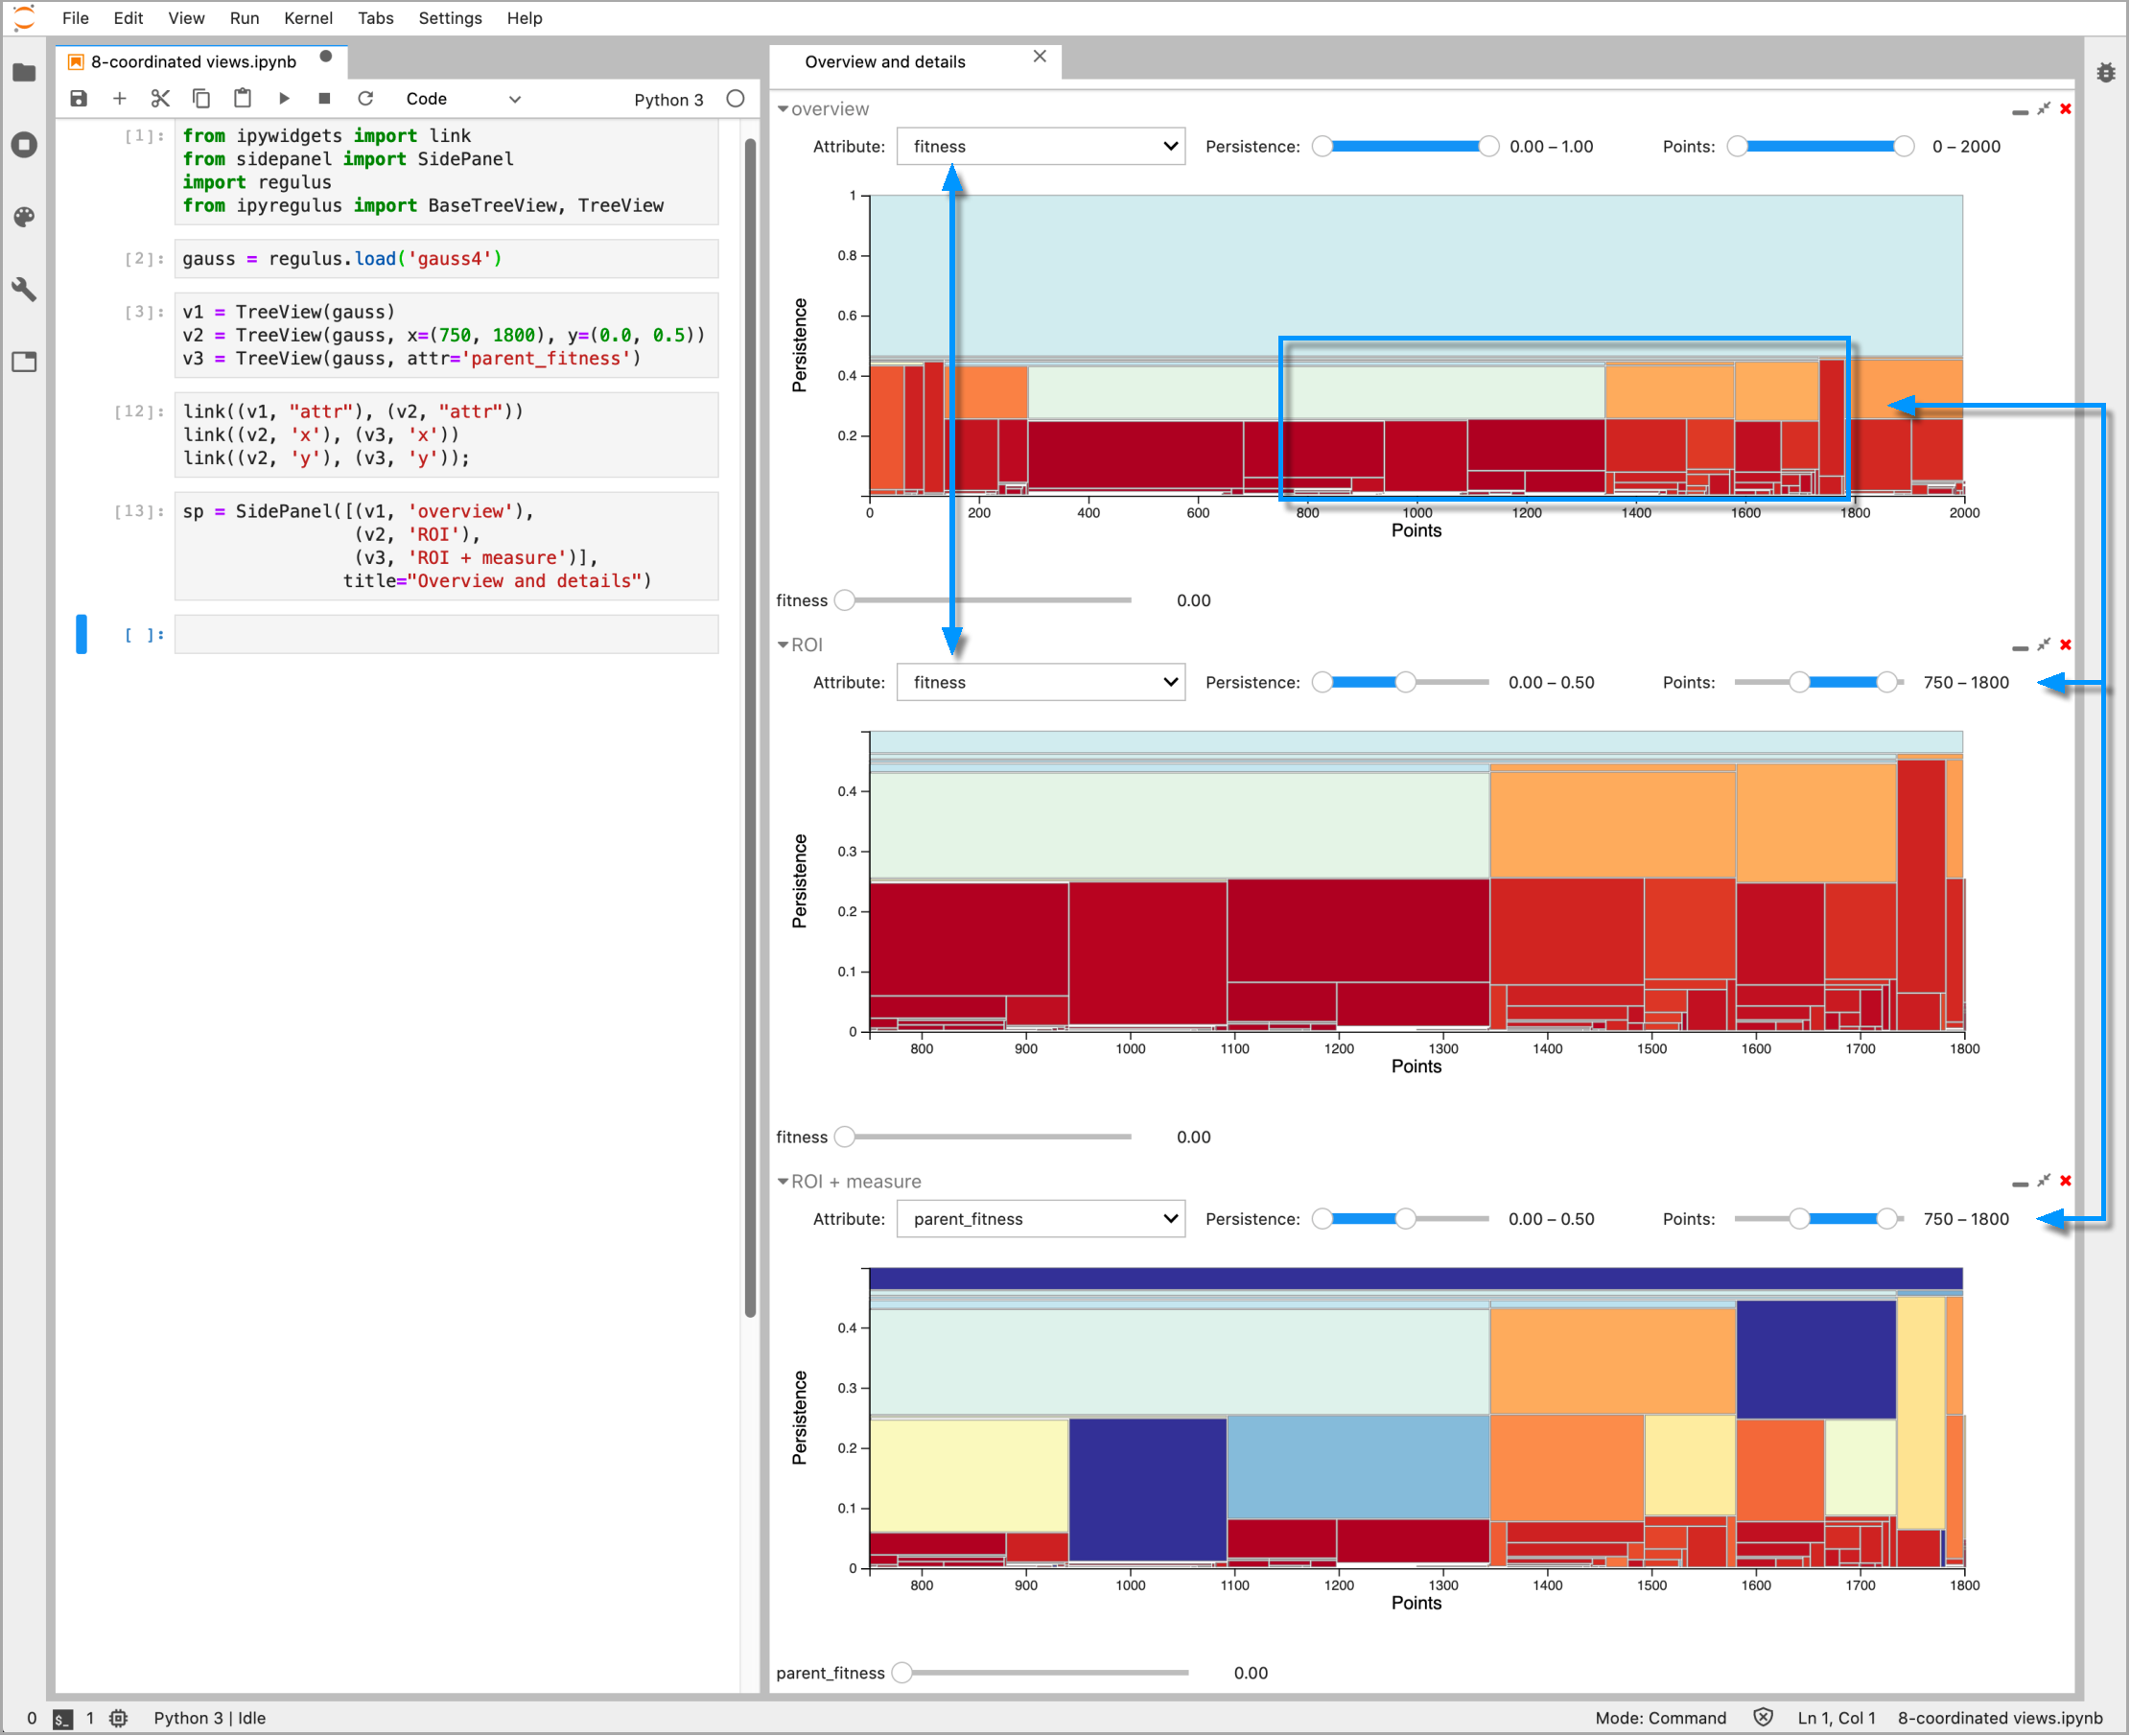
\includegraphics[width=\linewidth]{cmv}
    \caption{On the fly views coordination. Three views of the same tree in a SidePanel. Top and and middle views shows the same attribute (fitness) while the middle and bottom show the same region of interest. Changing the ROI in the middle or bottom views will update the other view.} 
    \label{fig:cmv}
    \end{center}
\end{figure}

\subsubsection{Tree Dependency}
\label{sec:tree-dependency}

Instead of explicit dataflow model with modules and ports.

\vspace{-.1in}
\section{Use Cases}
\label{sec:use_cases}

\subsection{Combustion}
\label{sec:combustion}
In this example we look at sample data extracted from a time dependent jet simulations of turbulent CO/H2-air flame, where each sample point consists of chemical composition and temperature~\cite{hawkes07}. The data includes extinction and reignition phenomena where several chemical components form and evolve during the combustion reaction and in turn effect the amount of heat released. In this analysis we explore the temperature in relation to the chemical composition. 

The data consist of 5172 samples with 10 chemical species. \autoref{fig:combustion-init}, depicts fitness for a \RT after filtering out partitions with less then 100 data points. The root of the tree demonstrates that a single linear model describe the whole data with an exceptional score of 0.998. We fit good models in most other partitions but they are not necessarily similar to each other. A zoom-in to persistence range [0, 0.15] (middle) reveals a large partition containing 30\% of data points all of which lie outside of the active combustion zone and should have been removed. This fact wasn't noticed in previous works. 

\begin{figure}[b]
    \begin{center}
     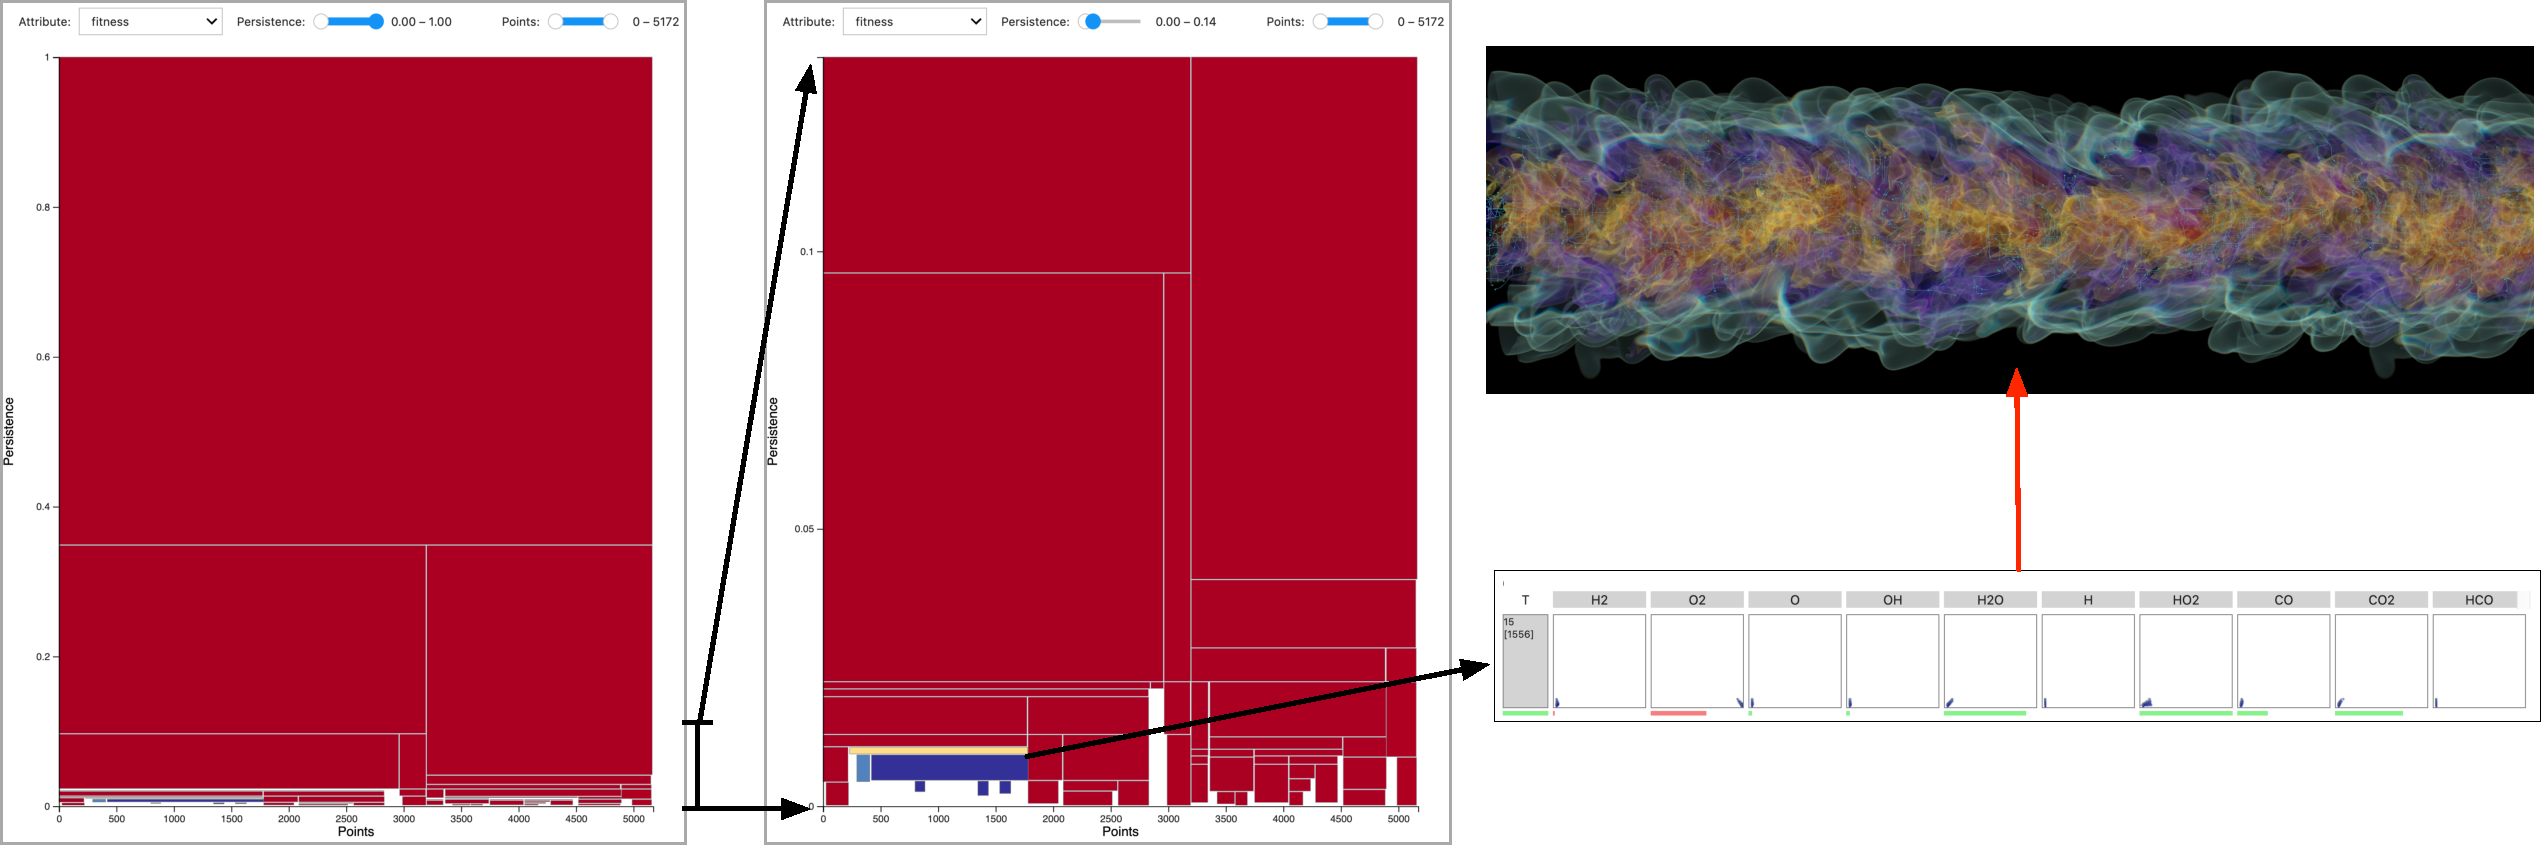
\includegraphics[width=\linewidth]{combustion-init-2}
     \vspace{-.2in}
    \caption{Combustion: Initial tree (left) shows that a single linear model describes all the data points(score = 0.998). Right: a zoom to persistence range [0:0.15] reveal a previously unknown partition containing large number (~30\%) of sample points that are outside of the active combustion zone and should have been removed (top).}
    \label{fig:combustion-init}
    \end{center}
         \vspace{-.1in}
\end{figure}

Using child and parent fitness doesn't reveal much but once we switch to child dimension fitness the tree comes to life, \autoref{fig:teaser}. The figure also shows the data points of the (four) top-most partitions that are different than their parents. Partition 494 (right most in the tree, bottom in the grid) is distinctly different from the other partitions. The three other partitions  differ mainly with respect of HO2, though the points in the first and third partitions (5 and 488) are mostly in the lower value. \autoref{fig:combustion-projections} shows the critical points graph. Note that the edges for the first three partitions overlap in (b) but are clearly separated in (c). 

The four partitions share a single maxima but feature four distinct minima. The minima in partition 494 captures a situation where fuel (H2 and CO) is available but the lack of oxidizer (O2) prevents a chemical reaction. The situation is reversed in partition 5 where oxidizer (O2) is available but the lack of fuel prevents a reaction. In partitions 460 and 488, the mixing of fuel and oxidizer is highly turbulent and blows the flames out, resulting in large amount of HO2. The clear separation between these two minima could be due to undersampling or possible the boundary of the manifold. 

% Originally only two minima were known and the third was discovered in an earlier work. The black annotation curve in (d) marks a possible boundary of the manifold, which may explain the three distinct minima we find in this area. The notches in this boundary, however, could also be due to undersampling. In contrast to the earlier work where the third minima was discovered after an exhaustive search through many potential simplifications and possible partitions, we were able to discover all four minima after a just a few steps in addition to identifying the invalid points. 

\begin{figure}[tb]
    \begin{center}
     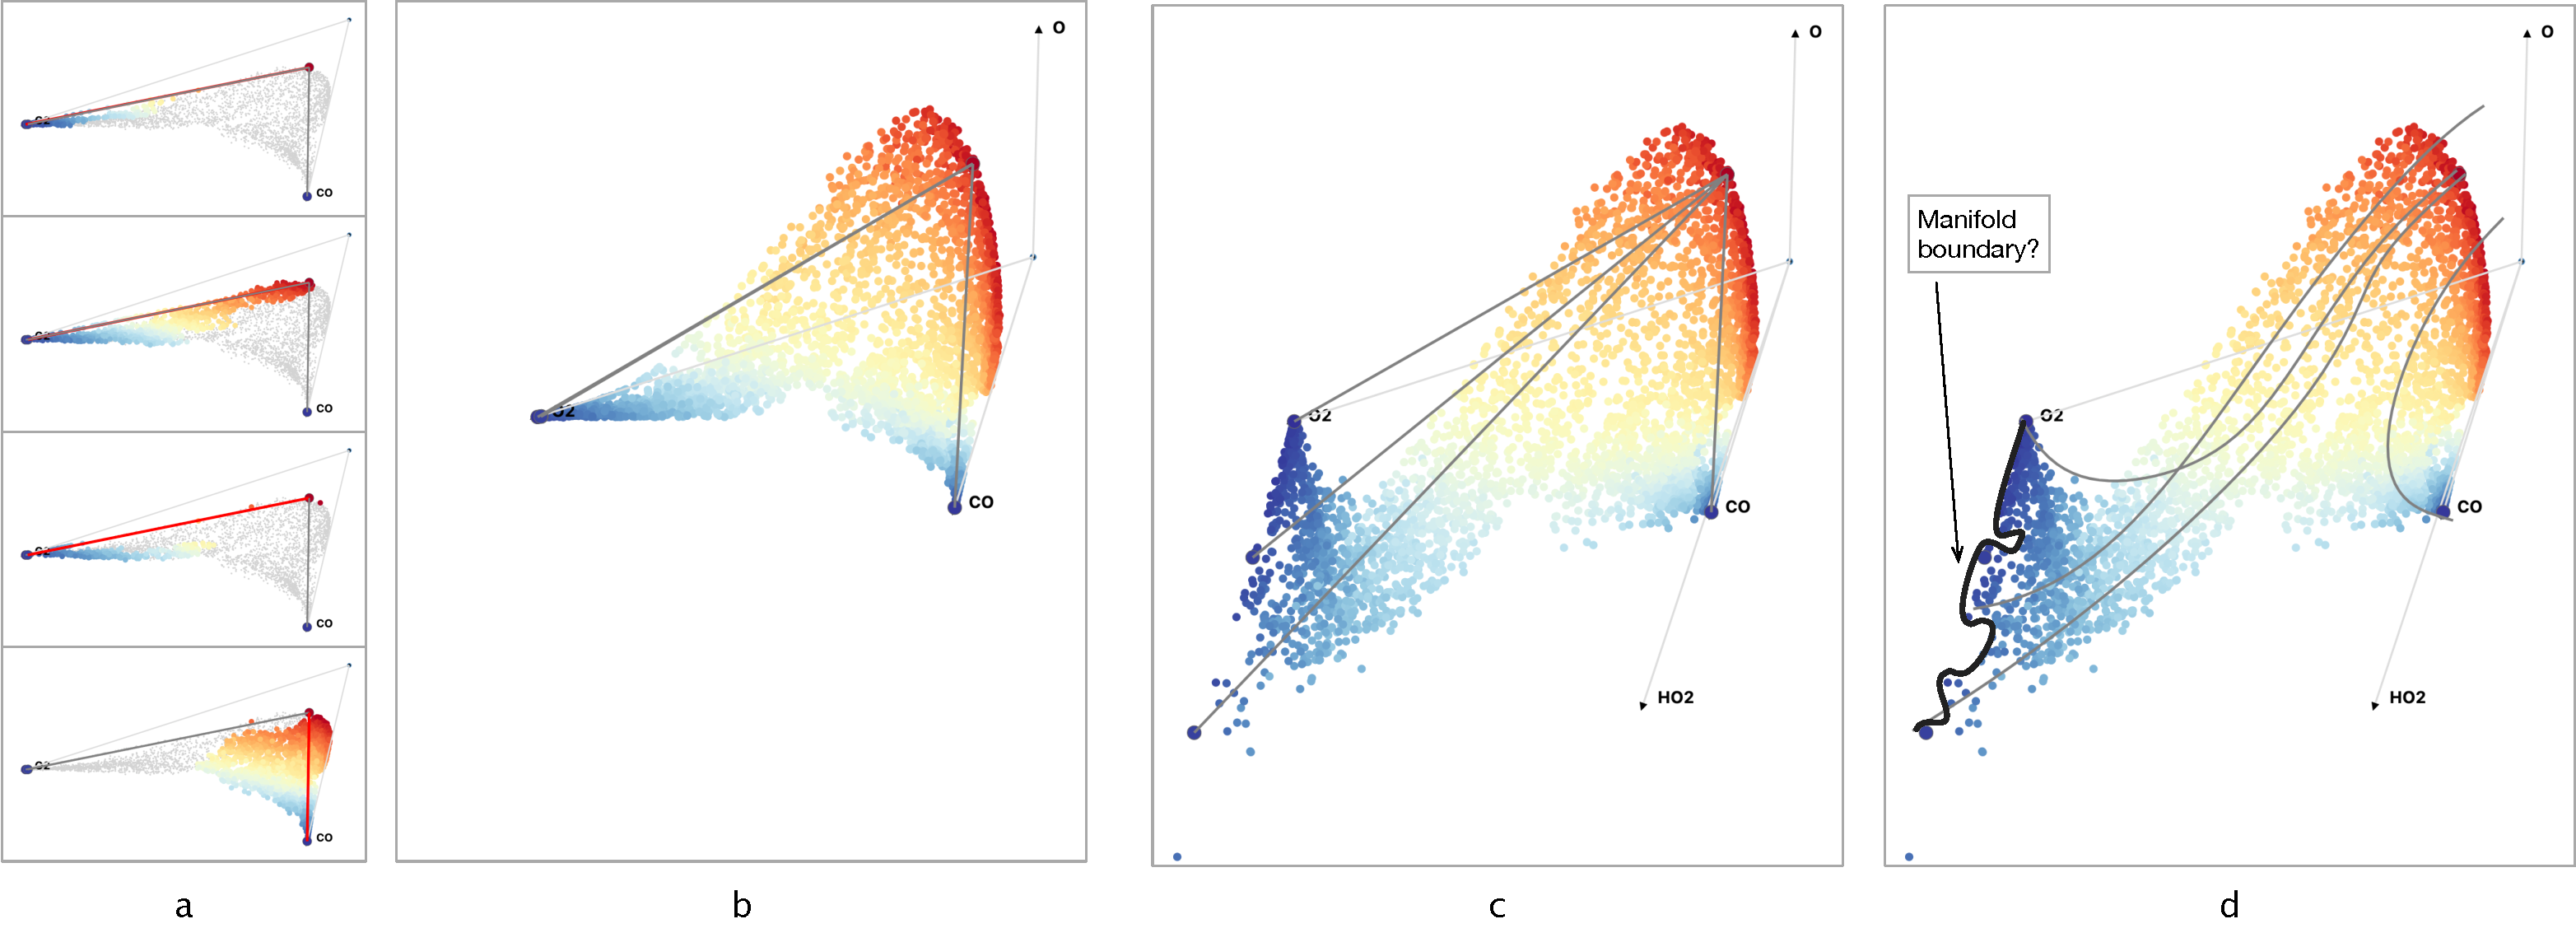
\includegraphics[width=\linewidth]{combustion-projections2}
             \vspace{-.1in}
    \caption{Graph views of the combustion data. a) Highlighting the points of each partition. b) Without the HO2 only the two expected minima are apparent. c) The three minima separates along the HO2 direction. d) Regression curves follow the shape of the manifold.}
    \label{fig:combustion-projections}
         \vspace{-.1in}
         \end{center}
\end{figure}

\subsection{Nuclear Fuel Cycle Simulations}
\label{sec:nuclear}
Nuclear fuel cycle analysis focuses on modeling the nuclear industry and ecosystem at a macroscopic level. This example studies scenarios for transitioning from one technology, Light Water Reactors (LWR) to a newer Sodium-cooled Fast breeder Reactor (SFR) technology. LWR reactors can use either enriched uranium (UOX, Uranium Oxyde) or a mixture of Uranium and Plutonium (MOX, Mixed Oxyde) as fuel but produce Minor Actinides waste. Minor Actinides have a long lifetime and high activities, which make such wastes  difficult to deal with. In contrast, SFR reactors mainly use a mix of Natural Uranium and Plutonium as a fuel (MOX). The SFR reactors have the ability to breed Plutonium from the Uranium and energy production is based on the fission of the Plutonium. This breeding capability allows the fuel to stay longer in the fuel, reducing the amount of Minor Actinides ultimately present in the waste. Some combination of fuel and SFR reactor configuration allows to breed more Plutonium than it will burn . A sufficiently large number of SFR reactors (used in 'breeder' configuration) can thus be self sustained.

\begin{figure}[b]
    \begin{center}
     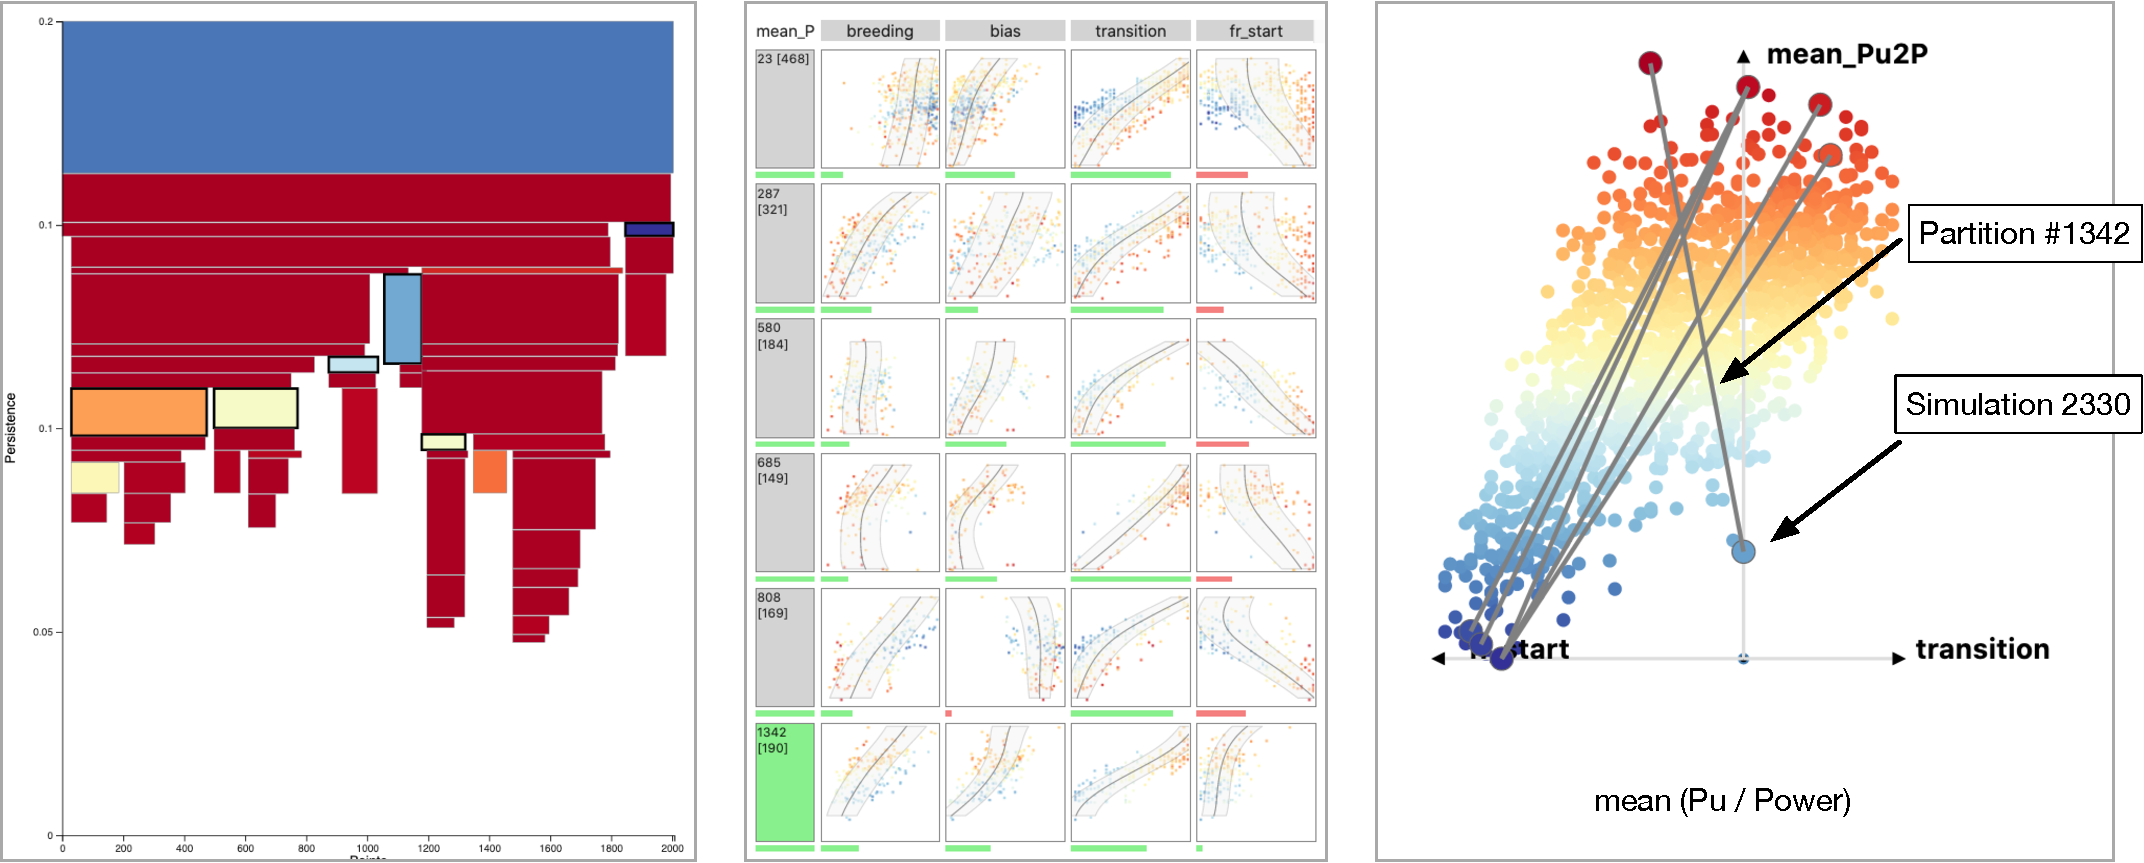
\includegraphics[width=\linewidth]{transition1}
    \caption{Transition scenario: Partitions selected based on dimension fitness (left). Partition 1342 exhibits unique behaviour (mid and right) though its minimum (simulation 2330) is not the lowest (right).}
        \vspace{-.1in}
    \label{fig:transition}
    \end{center}
\end{figure}

\begin{figure}[tb]
    \begin{center}
    \vspace{-.1in}
     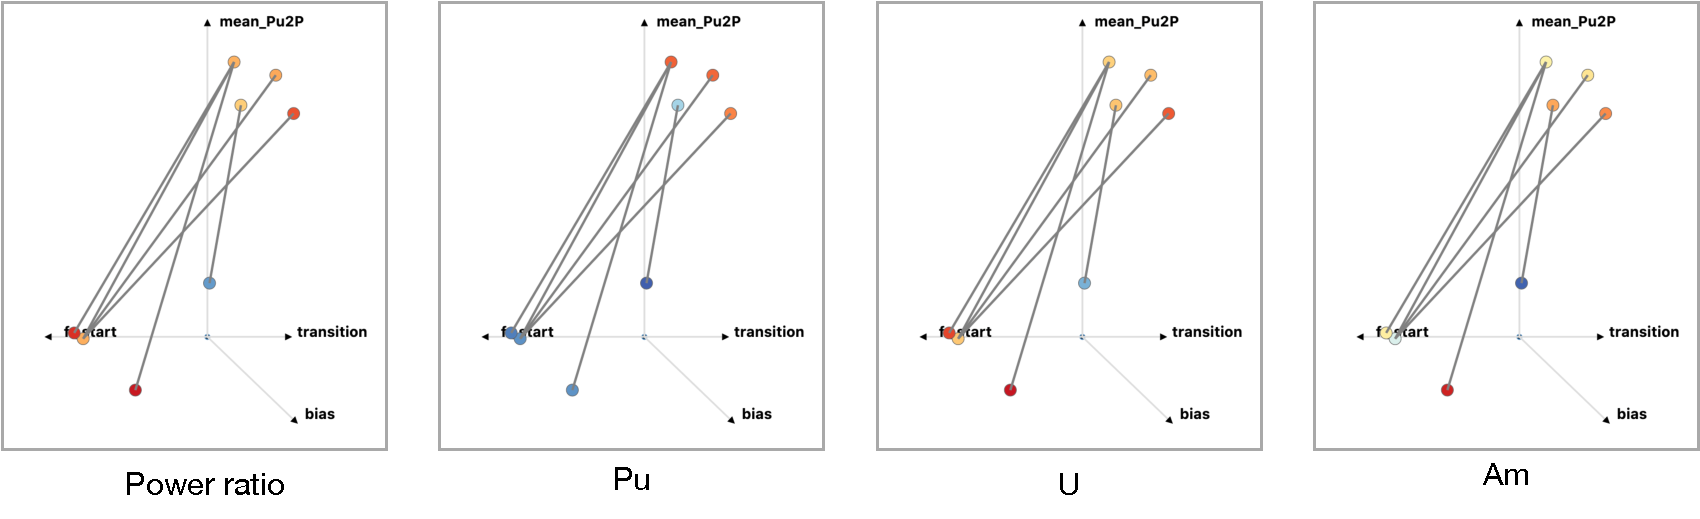
\includegraphics[width=\linewidth]{transition-graph1}
    \caption{Encoding other output variables as color demonstrates the advantages of simulation 2330 which exhibits low power ration and consistently generates low volumes of excess radio active materials.}
    \label{fig:transition-graph}
    \end{center}
\end{figure}

\begin{figure}[tb]
    \begin{center}
     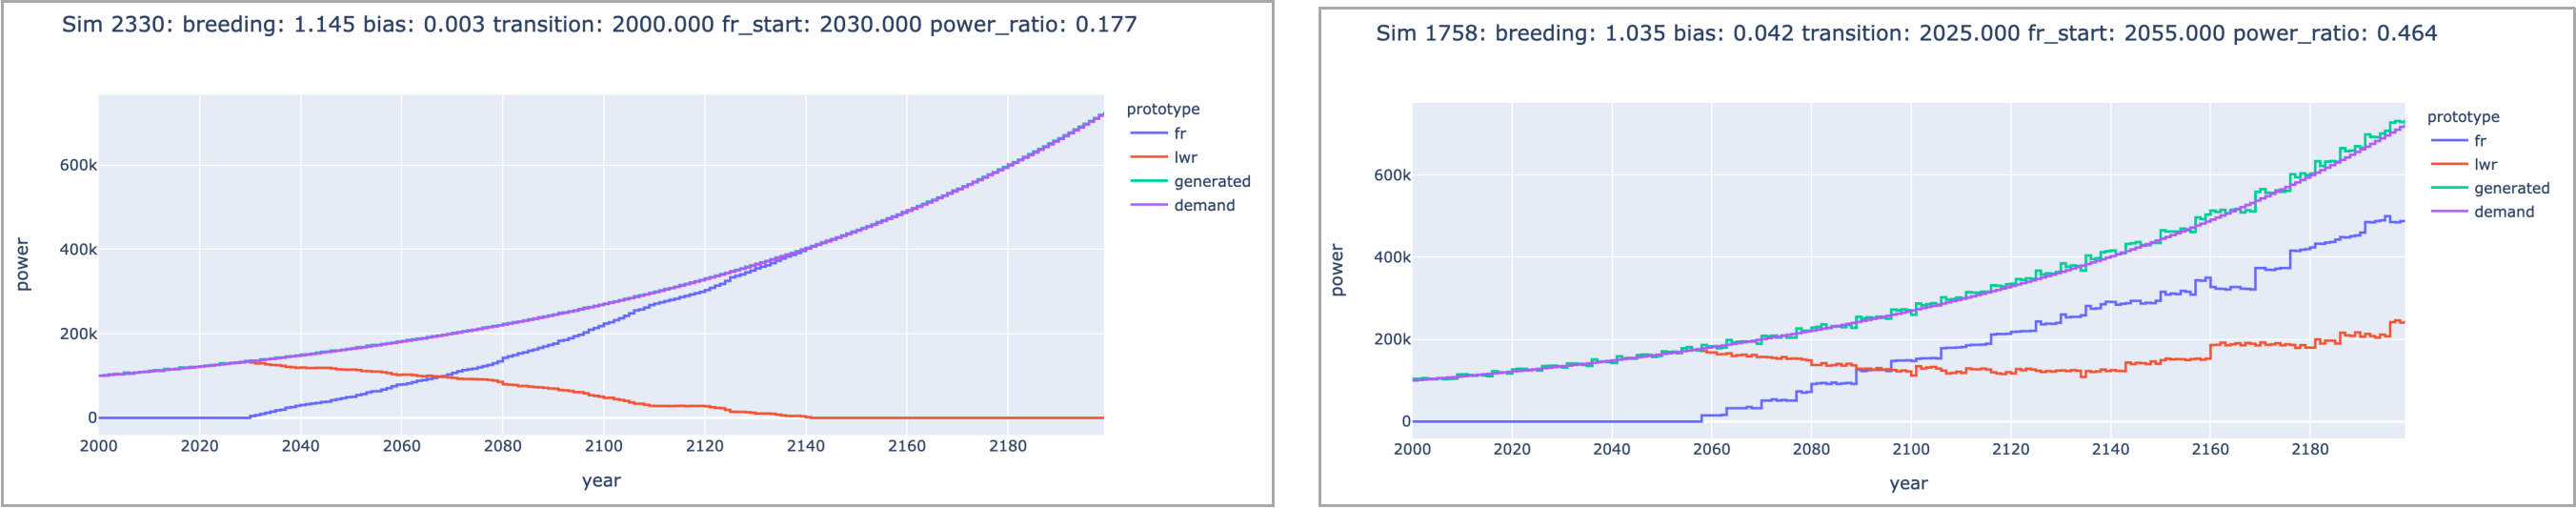
\includegraphics[width=\linewidth]{transition-plots-1}
    \caption{Simulation 2330 exhibits an excellent and smooth transition (left), while simulation 1758 does not lead to a transition (right).}
    \label{fig:transition-plots}
    \end{center}
\end{figure}

The study consists of 3300 simulation runs, using four input parameters (breeding ratio, start year of LWR fuel reprocessing, first year an SFR can be deploy and a bias measure). The aim here is to find a deployment schedule that transitions from an ecosystem consisting of LWRs to one with only SFR reactors, while minimizing some objective function. To this end we computed several objective functions at the end of each simulation including: the ratio of total power generated by LWRs reactors to the total energy generated over the simulation's 200 years span, the mean ratio of plutonium to generated power, and amount of nuclear waste such as Plutonium, Uranium and Americium. 
Of the 3300 simulation only 2007 led to a complete transition within the first 120 years). In the following we looked at the mean ration of Plutonium to power objective function. \autoref{fig:transition} show a reduced \RT (remove partitions with less than 100 simulations or a lifespan less then 0.001) depicting child dimension fitness. Several partitions that stand out are also shown. The graph view on the right shows that partition 1342 exhibits a unique behaviour, although its minima (simulation run 2330) doesn't have the lower value. \autoref{fig:transition-graph} shows that adding 'bias' in the graph view affects only one of the minima. However, when we use the same partitions and graph, but change the colors to encode other output values, we can see that simulation 2330 is unique in that it consistently exhibits low values (blues) for power ration and the amount of the nuclear waste generated. \autoref{fig:transition-plots} shows the deployment schedule of simulation 2330 (top) and an example of a simulation that doesn't lead to a complete transition. 
 


% \todo[inline]{Linear models in multi-dimensional may not be intuitive, for example the fr\_start in the transition use-case}
\section{Conclusions}
\label{sec:conclusions}
The \RT addresses the important, though often neglected, 'why' question by  proposing a new perspective of the topology simplification process. The \RT visualization offers both a concise broad view of the simplification landscape and a guide for an interactive visual exploration of the underlying scalar function. We describe the \RT in the context of Morse-Smale complexes, but the partition's perspective and the tree are equally applicable to Morse complexes. Some of the measures as well as the inverse regression curves are not directly applicable and one will have to use high order regression models.

The \RT has several limitations. First, it does not preserve spatial locality or even adjacency relation between partitions. Mapping spatial locality is a complex issue for multi-dimensional data in general. Adjacency information can be retrieved from the Morse-Smale complexes, though how to depict it is not clear and is especially problematic in a setting with many levels of details. 
Second, Morse-Smale partitions can have complex twisting shapes that are not captured directly in the tree structure and the tree does not address the notion of topological holes. 

We have begun exploring methods for using the inverse regression curves to facilitate adaptive sampling, both for validation purposes and for improving spatial resolutions in areas that are undersampled. We are also looking at using t-SNE and other dimensional reduction and clustering techniques to analyze the linear models and provide additional measures for identifying and highlighting potential unique partitions.

% \section{Acknowledgments}
% This work was funded in part by the U.S. Department of Energy, Nuclear Energy University Program (NEUP) grant DE-NE0008587.


%% if specified like this the section will be committed in review mode
\acknowledgments{
The authors wish to thank A, B, and C. This work was supported in part by
a grant from XYZ (\# 12345-67890).}

%\bibliographystyle{abbrv}
\bibliographystyle{abbrv-doi}
%\bibliographystyle{abbrv-doi-narrow}
%\bibliographystyle{abbrv-doi-hyperref}
%\bibliographystyle{abbrv-doi-hyperref-narrow}

\bibliography{paper}
\end{document}
